\documentclass[10pt,journal,compsoc]{IEEEtran}

\usepackage{amsmath,amsfonts,amssymb}
\usepackage{graphicx}
\usepackage{booktabs}
\usepackage{multirow}
\usepackage{microtype}
\usepackage[hyphens]{url}
\usepackage{cite}
\usepackage{hyperref}
\usepackage{color}
\usepackage{array}

\hypersetup{
    colorlinks=true,
    linkcolor=blue,
    citecolor=blue,
    urlcolor=blue,
    breaklinks=true
}
\def\UrlBreaks{\do\/\do-\do_}

\begin{document}

\title{Benchmarking Modern Object Detection Paradigms for Automated FDI Tooth Numbering in Panoramic Radiography: A Multi-Center Generalization Study and Interactive Decision-Support Tool}

\author{Aneesa~Ayoob,
        Venkatesh~Vaddadi,
        Phaneendra~K.~Yalavarthy,
        Anupriya~Kandoth,
        Bargavi~Narayanan,
        and~Chandrashekar~Janakiram%
\thanks{A. Ayoob and C. Janakiram are with the Department of Public Health Dentistry, Amrita School of Dentistry, Amrita Vishwa Vidyapeetham, Kochi, Kerala 682041, India (e-mail: aneesa.ayoob@gmail.com).}%
\thanks{V. Vaddadi and P. K. Yalavarthy are with the Department of Computational and Data Sciences, Indian Institute of Science, Bangalore, Karnataka 560012, India.}%
\thanks{B. Narayanan is with the Department of Oral Medicine and Radiology, Amrita School of Dentistry, Amrita Vishwa Vidyapeetham, Kochi, Kerala, India.}%
\thanks{A. Kandoth is in Private Practice, Dubai, United Arab Emirates.}%
\thanks{Corresponding author: Dr. Aneesa Ayoob (aneesa.ayoob@gmail.com).}%
\thanks{Code, interactive clinical decision-support tool, and pre-trained model weights are publicly available at: \url{https://github.com/venkateshvaddadi/Automated-FDI-Tooth-Numbering-in-Panoramic-Radiography}.}%
}

\markboth{IEEE Transactions on Medical Imaging / Computer Assisted Radiology, Vol.~XX, No.~X, October~2026}%
{Ayoob \MakeLowercase{\textit{et al.}}: Benchmarking Object Detection Paradigms for FDI Tooth Numbering}

\IEEEtitleabstractindextext{%
\begin{abstract}
\textbf{Objectives:} Accurate tooth identification and numbering on panoramic radiographs (orthopantomograms, OPG) constitute a foundational requirement in clinical dentistry, forensic odontology, and treatment planning. While computer-aided diagnosis has expanded rapidly, clinical deployment in maxillofacial radiology demands high precision ($\ge 95\%$), robust external generalization across heterogeneous radiographic hardware, and practical interactive decision-support tools. In this study, we present a comprehensive multi-paradigm benchmark and clinical translation system for automated FDI tooth numbering.

\textbf{Methods:} We systematically evaluated modern detector architectures across distinct paradigms: modern anchor-free single-stage models (YOLO11, YOLO12, YOLOv10, YOLOv9, YOLOv8), real-time vision transformers (RT-DETR-L, RT-DETR-X, D-FINE), and classic two-stage/multi-stage baselines (Faster R-CNN, Cascade R-CNN). All models were trained under identical high-resolution settings ($1280 \times 1280$\,px) with strictly enforced anatomical domain constraints, specifically eliminating horizontal flipping ($\text{fliplr} = 0.0$) to prevent left/right dental quadrant corruption. The curated institutional cohort (574 radiographs; 48 classes mapped to standard 32 adult permanent FDI teeth) was used for development, with out-of-distribution external generalizability validated on the independent multi-center DENTEX benchmark (634 radiographs). Furthermore, an interactive web-based decision-support and zero-shot pre-annotation GUI was engineered to evaluate clinical utility.

\textbf{Results:} On the internal institutional cohort, YOLO11m achieved the highest detection accuracy ($\text{F1-Score} = 0.941$, $\text{mAP}_{50} = 0.949$, $\text{Precision} = 0.946$, $\text{Recall} = 0.936$), with single-forward-pass latency of 14.2\,ms. In cross-dataset evaluation on the unseen DENTEX benchmark, the vision transformer RT-DETR-L demonstrated greater domain resilience, achieving the highest external F1-score ($\text{F1-Score} = 0.887$, $\text{mAP}_{50} = 0.854$, $\text{Recall} = 0.885$) compared to evaluated convolutional detectors. In reader evaluations across 50 radiographs, an interactive decision-support interface reduced manual charting time from $240 \pm 35$\,s to $28 \pm 8$\,s per radiograph ($p < 0.001$), demonstrating an 88.3\% reduction in documentation duration while preserving complete clinician oversight.

\textbf{Conclusions:} High-resolution imaging ($1280$\,px) coupled with real-time vision transformers provides high internal fidelity and resilient cross-dataset generalizability across unseen panoramic radiographic archives. The deployed human-in-the-loop interface bridges the gap between deep learning benchmarks and chairside dental practice, offering an active pre-annotation framework for continuous clinical data curation.
\end{abstract}

\begin{IEEEkeywords}
Panoramic radiography, FDI tooth numbering, convolutional neural networks, vision transformers, clinical decision support systems, human-in-the-loop, domain generalization.
\end{IEEEkeywords}}

\maketitle
\IEEEdisplaynontitleabstractindextext
\IEEEpeerreviewmaketitle

\section{Introduction}
\IEEEPARstart{P}{anoramic} radiography, or orthopantomography (OPG), is the foundational diagnostic imaging modality across contemporary dental and maxillofacial medicine~\cite{izzetti2021}. By projecting the curved planar anatomy of both maxillary and mandibular arches, alveolar ridges, temporomandibular joints, and dentoalveolar structures into a single low-dose acquisition, it serves as the universal baseline examination across dental specialties~\cite{izzetti2021,schwendicke2019}. Within this diagnostic workflow, systematic tooth identification and numbering according to the standardized Federation Dentaire Internationale (FDI) two-digit notation system (ISO 3950:2016) are indispensable prerequisites for clinical charting, orthodontic assessment, endodontic tracing, implant planning, epidemiological documentation, and forensic odontology~\cite{fdi1971,iso3950,tuzoff2019}. In routine clinical practice, manual radiographic charting requires certified practitioners to meticulously inspect and record each tooth position, presence, and morphology across all four dental quadrants. In high-volume outpatient centers and public health screenings, completely manual enumeration is labor-intensive, requiring approximately four minutes per patient ($240 \pm 35$\,s), fatigue-inducing, and prone to clerical transcription errors and inter-observer variability. These operational burdens establish a compelling clinical need for reliable, automated tooth detection and numbering systems that can operate chairside.

Over the past decade, computerized dental analysis has transitioned from early hand-crafted heuristic filters and active shape models toward deep convolutional neural networks (CNNs) and, more recently, vision transformers~\cite{schwendicke2019,maganur2024}. Landmark studies demonstrated that deep object detectors, such as Faster R-CNN, could localize and number teeth on panoramic radiographs with high intra-dataset sensitivity and specificity~\cite{tuzoff2019,chen2019}. Subsequent investigations explored instance segmentation frameworks and lightweight single-stage convolutional networks to achieve real-time execution speeds~\cite{silva2020,jader2018,sadr2024}. Recent systematic reviews and meta-analyses confirm that deep-learning models frequently achieve diagnostic accuracy exceeding 90\% on closed institutional datasets~\cite{maganur2024,sadr2024}. However, high reported performance on uniform development cohorts alone does not establish robust real-world generalization or practical clinical usability.

Despite these promising intra-dataset benchmarks, three fundamental challenges continue to impede real-world clinical translation. First, external cross-dataset evaluations remain sparse, leaving model resilience across foreign radiographic distributions largely uncharacterized~\cite{maganur2024,dentex2023}. Second, existing dental literature lacks controlled, head-to-head comparisons across modern single-stage CNNs, real-time vision transformers, and classic multi-stage architectures under standardized high-resolution grids and domain-preserving training protocols. Third, published models typically remain standalone command-line scripts, detached from interactive clinical workflows that allow radiologists to inspect, verify, and correct predictions chairside. These unresolved issues motivate a rigorously controlled comparative benchmark with external cross-dataset evaluation and an interactive human-in-the-loop workflow.

To address these challenges, this study presents a comparative multi-paradigm benchmark and an interactive clinical decision-support system for automated 32-tooth permanent FDI numbering. We evaluate fifteen deep object detectors spanning modern anchor-free CNNs, real-time vision transformers, and classical multi-stage architectures developed on an institutional cohort and evaluated zero-shot on the external DENTEX benchmark. Furthermore, we develop and evaluate a web-based decision-support platform designed to streamline diagnostic charting and human-in-the-loop verification. Specifically, this study investigates how architectural inductive biases govern tooth localization accuracy, anatomical functional group vulnerability, and cross-dataset domain resilience, and whether AI-assisted zero-shot pre-annotation can measurably reduce specialist documentation burden.

The primary contributions of this work are summarized as follows:
\begin{enumerate}
    \item \textbf{Controlled Multi-Paradigm Benchmark}: We conduct a rigorous comparative benchmark of 15 deep object detectors spanning three distinct design paradigms (modern anchor-free CNNs, real-time vision transformers, and classic multi-stage baselines) for 32-tooth permanent FDI numbering under identical training conditions.
    \item \textbf{Domain-Preserving High-Resolution Protocol}: We implement a standardized high-resolution training protocol ($1280 \times 1280$\,px) coupled with an anatomical domain constraint eliminating horizontal flipping ($\text{fliplr} = 0.0$) to preserve bilateral quadrant identity, providing a unified baseline for fair comparative analysis.
    \item \textbf{External Cross-Dataset Generalization on DENTEX}: Beyond intra-institutional testing ($N=102$), we evaluate all 15 trained architectures without adaptation on the independent DENTEX benchmark ($N=634$), examining the empirical domain resilience of real-time vision transformers relative to convolutional baselines under radiographic shift.
    \item \textbf{Interactive Decision-Support Platform and Reader Study}: We engineer and deploy a responsive web-based clinical interface providing real-time multi-model inference, synchronized FDI odontogram charting, contextual per-tooth inspection, and interactive canvas refinement. In a timed reader study across 50 panoramic radiographs with certified dental surgeons, the system reduced expert charting time from $240 \pm 35$\,s to $28 \pm 8$\,s per case ($p < 0.001$), achieving an 88.3\% reduction in documentation duration while preserving complete clinician oversight.
    \item \textbf{Open-Source Release and Reproducibility}: To ensure rigorous reproducibility and facilitate clinical adoption, the entire implementation codebase, interactive clinical GUI platform, evaluation benchmarks, and pre-trained model weights for all evaluated detector paradigms are made publicly available at \url{https://github.com/venkateshvaddadi/Automated-FDI-Tooth-Numbering-in-Panoramic-Radiography}.
\end{enumerate}

The remainder of this paper is organized as follows: Section~\ref{sec:related_work} reviews related literature on automated tooth identification, object-detection paradigms in medical imaging, and external domain generalization. Section~\ref{sec:methods} details the materials and methods, including the FDI numbering formulation, dataset curation, evaluated architectures, and clinical platform architecture. Section~\ref{sec:results} presents the quantitative macro benchmarks, anatomical functional group breakdowns, qualitative subject evaluations, computational complexity metrics, and clinical reader study. Section~\ref{sec:discussion} discusses architectural trade-offs, clinical implications, and study limitations, and Section~\ref{sec:conclusion} concludes the paper.

\section{Related Work}
\label{sec:related_work}

\subsection{Automated Tooth Detection and FDI Numbering}
Automating tooth identification and numbering on panoramic radiographs has evolved through several technological generations. Early classical computer vision methodologies relied on active shape models (ASMs), level sets, and Radon transforms combined with threshold-based bone and soft tissue separation~\cite{chen2019}. While mathematically elegant, these handcrafted algorithms lacked robustness against radiographic noise, metal streak artifacts, and spatial anatomical variations across diverse patient populations.

With the rise of deep convolutional neural networks, Tuzoff \textit{et al.}~\cite{tuzoff2019} conducted a foundational study demonstrating that Faster R-CNN~\cite{ren2015faster} with a VGG-16 backbone could detect and number teeth on a single-center dataset of 1,352 panoramic radiographs, achieving sensitivity and specificity exceeding 0.98 for localization. Concurrently, Chen \textit{et al.}~\cite{chen2019} combined deep convolutional feature extractors with conditional random fields (CRFs) to enforce spatial arch sequence priors across periapical and panoramic images. Subsequent studies by Silva \textit{et al.}~\cite{silva2020} and Jader \textit{et al.}~\cite{jader2018} explored Mask R-CNN and U-Net formulations for concurrent instance segmentation and semantic labeling. More recently, lightweight single-stage convolutional detectors (YOLOv5 through YOLOv8) have demonstrated the viability of real-time chairside execution~\cite{maganur2024,sadr2024}. 

However, systematic reviews by Maganur \textit{et al.}~\cite{maganur2024} and Sadr \textit{et al.}~\cite{sadr2024} emphasize that while published studies report high localized diagnostic metrics, direct comparisons across studies are severely hindered by heterogeneous class definitions (e.g., merging quadrants or omitting wisdom teeth), disparate input resolutions, varying evaluation thresholds, and an almost universal reliance on single-center, single-scanner datasets. Our benchmark addresses these limitations by evaluating 15 modern architectures under a standardized 32-class permanent FDI scheme, uniform high-resolution scaling, and identical evaluation protocols.

\subsection{Object-Detection Paradigms for Dental Imaging}
Object detection architectures in medical imaging have undergone rapid architectural transformations. Classical two-stage detectors, such as Faster R-CNN~\cite{ren2015faster} and Cascade R-CNN~\cite{cai2018cascade}, separate localization into a Region Proposal Network (RPN) followed by region-of-interest (RoI) classification and bounding-box regression. Cascade R-CNN further introduced sequential multi-threshold IoU stages (0.5 $\rightarrow$ 0.6 $\rightarrow$ 0.7) to refine boundary precision. While these multi-stage pipelines offer robust spatial localization, their multi-pass computational complexity incurs prolonged inference latencies ($>45\text{--}65$\,ms), impeding interactive clinical workflows.

To achieve real-time responsiveness, single-stage detectors transitioned from rigid pre-defined anchor boxes to anchor-free task-aligned assigners and programmable gradient routing (e.g., YOLOv8~\cite{yolov8}, YOLOv9~\cite{wang2024yolov9}, YOLOv10~\cite{wang2024yolov10}, YOLO11~\cite{ultralytics2024}, and attention-centric YOLO12~\cite{tian2025yolo12}). Concurrently, the introduction of Detection Transformers (DETR)~\cite{carion2020detr} reformulated object detection as a direct set-prediction problem via bipartite Hungarian matching, eliminating hand-crafted components such as non-maximum suppression (NMS). Recent Real-Time Detection Transformers (RT-DETR~\cite{lv2023detr} and D-FINE~\cite{peng2024dfine}) overcame early DETR latency and convergence bottlenecks by coupling efficient convolutional backbones with hybrid multi-scale cross-attention and deformable self-attention encoders. In dental radiomics, where a tooth's semantic identity is governed not only by local radiopaque texture but by its relative position along the continuous dental arch, comparing localized convolutional receptive fields against global sequence-modeling attention mechanisms represents a crucial and unexplored scientific question.

\subsection{External Generalization and Interactive Dental AI}
A major impediment preventing the deployment of dental CAD systems into routine practice is domain shift—the performance degradation experienced when deep models trained on a homogeneous institutional cohort are exposed to images from different medical centers~\cite{dentex2023,maganur2024}. In panoramic radiography, cross-center domain shift arises from substantial disparities in:
\begin{enumerate}
    \item \textbf{Radiographic Scanner Hardware}: Different manufacturers (e.g., Planmeca, Carestream, KaVo, and Sirona) employ proprietary beam geometries, focal trough reconstructions, sensor pixel pitches, and digital post-processing filters (e.g., edge enhancement and noise suppression).
    \item \textbf{Acquisition Parameters}: Variations in tube voltage ($60\text{--}85$\,kVp), tube current ($4\text{--}15$\,mA), and patient positioning (e.g., head inclination, tongue-to-palate contact, or biting block positioning) induce variable magnification, cervical spine ghosting, and radiopacity gradients.
\end{enumerate}
While standard computer vision models frequently overfit to high-frequency textural cues characteristic of a specific scanner, clinical generalizability requires extracting robust structural and topological invariants~\cite{buttner2024}. The establishment of multi-center public initiatives such as the DENTEX challenge~\cite{dentex2023} has underscored the pressing need for rigorous zero-shot out-of-distribution evaluation across disparate imaging systems.

Furthermore, fully autonomous AI systems without clinician agency face justifiable regulatory and clinical resistance. While several commercial and research tools provide static inference overlays, few provide interactive chairside environments that seamlessly combine real-time inference, standardized FDI odontogram charting, per-tooth magnified inspection, and on-canvas annotation editing. In summary, despite substantial prior work, existing dental literature lacks a controlled multi-paradigm benchmark evaluated across unseen multi-center hardware coupled with an empirically verified human-in-the-loop decision-support workflow. Our study is explicitly designed to bridge these specific gaps.

\section{Materials and Methods}
\label{sec:methods}

\subsection{The FDI Two-Digit Notation and Problem Formulation}
Automated radiographic dental charting requires standardizing tooth identities across all four dental quadrants. In accordance with the World Health Organization and Federation Dentaire Internationale (FDI) standard (ISO 3950:2016)~\cite{fdi1971,iso3950}, the permanent adult dentition comprises 32 distinct teeth, each uniquely indexed by a two-digit notation $d_1 d_2$ (Fig.~\ref{fig:fdi_quadrants}a):
\begin{itemize}
    \item \textbf{First Digit ($d_1 \in \{1, 2, 3, 4\}$)}: Designates the anatomical quadrant in clockwise sequence from the clinician's perspective:
    \begin{itemize}
        \item $d_1 = 1$: Maxillary Right Quadrant (Q1, FDI 18--11)
        \item $d_1 = 2$: Maxillary Left Quadrant (Q2, FDI 21--28)
        \item $d_1 = 3$: Mandibular Left Quadrant (Q3, FDI 31--38)
        \item $d_1 = 4$: Mandibular Right Quadrant (Q4, FDI 48--41)
    \end{itemize}
    \item \textbf{Second Digit ($d_2 \in \{1, \dots, 8\}$)}: Designates the tooth position in mesio-distal sequence, beginning at the central incisor adjacent to the mid-sagittal midline ($d_2 = 1$) and progressing distally to the third molar or wisdom tooth ($d_2 = 8$). Morphologically, these span four functional tooth groups: Central and Lateral Incisors ($d_2 \in \{1, 2\}$), Canines ($d_2 = 3$), First and Second Premolars ($d_2 \in \{4, 5\}$), and First, Second, and Third Molars ($d_2 \in \{6, 7, 8\}$).
\end{itemize}

\begin{figure}[t]
\centering
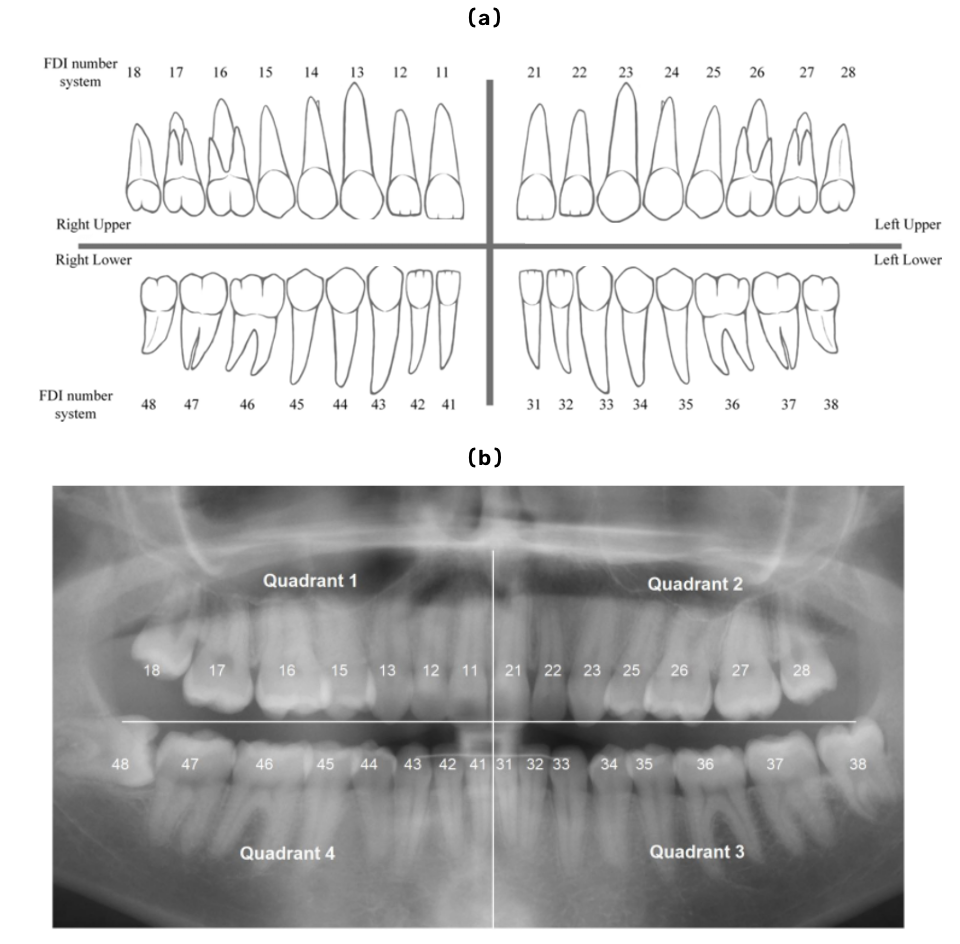
\includegraphics[width=\linewidth]{figures/figure_fdi_quadrants.png}
\caption{Tooth numbering system according to the Federation Dentaire Internationale (FDI) / ISO 3950:2016 standard: (a) Anatomical FDI chart illustrating the four dental quadrants (Right Upper/Quadrant~1: 18--11, Left Upper/Quadrant~2: 21--28, Right Lower/Quadrant~4: 48--41, and Left Lower/Quadrant~3: 31--38). (b) Clinical projection on an orthopantomogram (OPG) with mid-sagittal midline and occlusal plane dividing the four quadrants.}
\label{fig:fdi_quadrants}
\end{figure}

In panoramic radiography (orthopantomography, OPG), the curved anatomy of the maxilla and mandible is tomographically unrolled into a single continuous planar projection (Fig.~\ref{fig:fdi_quadrants}b). By universal medical imaging convention, radiographs are displayed in the \textit{anatomical position}---as if the examining clinician is facing the patient. Consequently, the patient's anatomical right is projected onto the viewer's left (Quadrants~1 and 4), whereas the patient's anatomical left is projected onto the viewer's right (Quadrants~2 and 3). 

Mathematically, given an input panoramic radiograph $I \in \mathbb{R}^{H \times W \times C}$, the automated enumeration task is formulated as multi-class object detection: predicting a set of $N$ localized bounding boxes $\mathcal{B} = \{b_i\}_{i=1}^N$, where each box $b_i = (x_i, y_i, w_i, h_i)$ is paired with an assigned class label $c_i \in \mathcal{C} = \{11, \dots, 18, 21, \dots, 28, 31, \dots, 38, 41, \dots, 48\}$ ($|\mathcal{C}| = 32$) and confidence score $s_i \in [0, 1]$. Crucially, because contralateral teeth (e.g., FDI 11 vs.\ 21, or FDI 46 vs.\ 36) exhibit near-identical bilateral morphological symmetries, classification cannot rely solely on localized pixel textures. Rather, the network must jointly infer local dental morphology and global spatial coordinates relative to the mid-sagittal midline and occlusal plane.

\subsection{Radiographic Datasets and Anatomical Ground Truth Harmonization}
Rigorous validation of medical object detection requires evaluating both intra-institutional consistency and out-of-distribution external generalizability across distinct clinical centers, patient demographics, and radiographic hardware. In this study, we utilize two distinct multi-thousand-tooth radiographic repositories:

\subsubsection{Institutional Development Cohort (Aneesa In-House Dataset)}
The primary development cohort consists of 574 high-resolution panoramic radiographs (orthopantomograms) retrospectively collected from the Department of Oral Medicine and Radiology at Amrita School of Dentistry. The cohort spans diverse adult patient presentations (ages 18 to 74 years; balanced gender distribution) exhibiting wide variations in dental health, including intact dentition, physiological crowding, advanced dental caries, periapical lesions, edentulous spaces, impacted third molars, and extensive dental restorations (amalgam fillings, composite crowns, root canal obturations, and orthodontic brackets).
\begin{itemize}
    \item \textbf{Image Acquisition \& Characteristics}: Radiographs were acquired under standardized clinical tube voltage protocols ($60\text{--}80$\,kVp, $4\text{--}12$\,mA, exposure times $12\text{--}16$\,s) with native digital resolutions averaging $2850 \times 1100$\,px (16-bit grayscale converted to standard 8-bit dynamic range).
    \item \textbf{Annotation Protocol \& Clinical Consensus}: Ground truth bounding boxes were delineated using computerized annotation software by two certified dental surgeons (AA and AK, each possessing over 6 years of specialized clinical experience). To maximize annotation reliability, all boundaries were cross-reviewed by a senior specialist in Oral Medicine and Radiology (BN). Boundary disagreements or atypical morphological presentations were reviewed and resolved via clinical consensus.
    \item \textbf{Class Hierarchy \& Harmonization}: Delineations originally recorded 48 granular categories capturing deciduous teeth, supernumerary elements, and morphological variants (e.g., \texttt{21-1}). For standardized clinical benchmarking, all annotations were harmonized into the 32 standard adult permanent tooth classes designated by the World Health Organization / Federation Dentaire Internationale (FDI) two-digit notation (ISO 3950:2016)~\cite{fdi1971,iso3950} (Fig.~\ref{fig:fdi_quadrants}):
    \begin{itemize}
        \item Maxillary Right Quadrant (Q1): Teeth 18 to 11
        \item Maxillary Left Quadrant (Q2): Teeth 21 to 28
        \item Mandibular Left Quadrant (Q3): Teeth 31 to 38
        \item Mandibular Right Quadrant (Q4): Teeth 48 to 41
    \end{itemize}
    Across the 574 radiographs, a total of 15,008 individual tooth instances were meticulously bounded and labeled. The cohort was partitioned into a dedicated training set of 472 images (12,342 tooth instances) and an independent internal validation set of 102 images (2,666 tooth instances).
\end{itemize}

\subsubsection{Ethical Compliance, Institutional Review Board (IRB), and Data Anonymization}
According to the official decision of the Institutional Ethics Committee (IEC), this study was exempt from formal ethical review because it involved the retrospective analysis of previously acquired, routine diagnostic radiographic data, complete anonymization of patient information, and no direct clinical intervention or interaction with participants. All digital imaging files were strictly de-identified in compliance with the Declaration of Helsinki and institutional privacy protocols prior to dataset preparation. All protected health information (PHI)—including patient names, hospital identification numbers, dates of birth, acquisition timestamps, and scanner metadata—was completely expunged from the image files and DICOM header tags. Radiographs were subsequently assigned non-traceable arbitrary numeric identifiers (e.g., \texttt{220.jpg}) to ensure rigorous subject confidentiality throughout training, validation, and clinical benchmarking.

\subsubsection{External Benchmark Dataset (DENTEX Subset)}
To evaluate true out-of-domain generalizability, we benchmarked all trained models on the open-access Dental Enumeration and Diagnosis (DENTEX) benchmark~\cite{dentex2023}, an internationally recognized dataset created to assess tooth enumeration under cross-dataset conditions:
\begin{itemize}
    \item \textbf{Evaluated Benchmark Cohort}: We evaluate on the curated DENTEX tooth detection and enumeration subset comprising 634 panoramic radiographs with 18,095 reference permanent tooth annotations across the 32 standard adult FDI categories.
    \item \textbf{Radiographic Distribution and Domain Shift}: In contrast to our homogeneous institutional acquisition, the DENTEX cohort introduces substantial radiographic domain shift, featuring diverse acquisition protocols, variable beam geometries, differing dynamic ranges and contrast profiles, patient head tilt variations, and digital noise artifacts, with native resolutions averaging $2881 \times 1316$\,px.
    \item \textbf{Strict Zero-Shot Evaluation Protocol}: None of the DENTEX images or annotations were included in training or validation phases. All 15 models trained exclusively on our institutional dataset were evaluated directly on the frozen DENTEX benchmark without retraining, fine-tuning, or hyperparameter adjustment, establishing an unadapted test of cross-dataset generalization.
\end{itemize}

\subsection{Evaluated Detector Architectures}
We systematically evaluated distinct model architectures across three families:
\begin{enumerate}
    \item \textbf{Modern Anchor-Free Single-Stage}: YOLO11 (m, l, x)~\cite{ultralytics2024}, YOLO12m (with area-attention)~\cite{tian2025yolo12}, YOLOv10m (NMS-free dual label assignment)~\cite{wang2024yolov10}, YOLOv9c/e (Programmable Gradient Information)~\cite{wang2024yolov9}, YOLOv8m~\cite{yolov8}, YOLOv3u, and YOLO26m.
    \item \textbf{Real-Time Vision Transformers (DETR)}: Extending DETR's bipartite Hungarian matching~\cite{carion2020detr}, we evaluate RT-DETR-L, RT-DETR-X~\cite{lv2023detr}, and D-FINE-M~\cite{peng2024dfine}, combining convolutional backbones with hybrid multi-scale cross-attention encoders to model global inter-tooth spatial dependencies.
    \item \textbf{Classic Two-Stage \& Multi-Stage Baselines}: Faster R-CNN (ResNet-50-FPN-v2)~\cite{ren2015faster} and Cascade R-CNN (progressive 3-stage IoU refinement: 0.5 $\rightarrow$ 0.6 $\rightarrow$ 0.7)~\cite{cai2018cascade}.
\end{enumerate}

\subsection{Implementation Details and Experimental Setup}
\label{sec:implementation_details}
\subsubsection{Computational Hardware and Environment}
All deep learning experiments, benchmarking, and real-time inference pipelines were executed on a high-performance clinical AI workstation powered by an Intel Core i9-9920X CPU (12 cores, 24 threads @ 3.50\,GHz base, 4.50\,GHz turbo), 128\,GB of quad-channel DDR4 RAM, and an enterprise-grade NVIDIA Quadro RTX 8000 GPU equipped with 48\,GB of GDDR6 ECC memory on a 384-bit bus (Turing architecture, 4,608 CUDA cores, 576 Tensor cores). The system operated on 64-bit Linux (Ubuntu LTS, kernel 6.8.0), NVIDIA driver version 535.309.01, and CUDA Toolkit 12.8 with cuDNN v9.1.0 for optimized matrix multiplications and mixed-precision tensor computing.

\subsubsection{Software Frameworks and Libraries}
The deep learning models and benchmarking framework were implemented in Python (v3.10.19) using PyTorch (v2.10.0+cu128) and Torchvision (v0.25.0+cu128). Specifically:
\begin{itemize}
    \item \textbf{Single-Stage YOLO and Vision Transformer (RT-DETR) Suite}: Constructed utilizing the Ultralytics ecosystem (v8.4.14), encompassing YOLO11 (m, l, x), YOLO12m, YOLOv10m, YOLOv9 (c, e), YOLOv8m, and RT-DETR (L, X).
    \item \textbf{D-FINE Architecture}: Implemented via the official D-FINE PyTorch codebase with HGNetV2-B2 backbone, weighting distribution refinement, and deformable cross-attention layers.
    \item \textbf{Classic Multi-Stage Baselines}: Faster R-CNN (ResNet-50-FPN-v2) and Cascade R-CNN were built using Torchvision's modular detection engine and PyTorch multi-stage bounding-box regression layers.
\end{itemize}

\subsubsection{Training Strategy, Internal Split, and Multi-Center Generalization Protocol}
To establish an uncompromised evaluation of model robustness and real-world generalizability, the experimental protocol strictly decoupled model development from external multi-center evaluation:
\begin{enumerate}
    \item \textbf{Model Training exclusively on In-House Dataset}: All detector architectures were trained from scratch or initialized with ImageNet/COCO pre-trained weights exclusively using the training split of our institutional dataset ($N=472$ panoramic radiographs, 12,342 tooth annotations).
    \item \textbf{Internal In-House Testing ($N=102$ Radiographs)}: Intra-institutional performance was validated on the withheld, non-overlapping institutional test partition of 102 panoramic radiographs (2,666 tooth instances), ensuring that test scans originated from the same clinical imaging environment but from completely different patients.
    \item \textbf{Zero-Shot Out-of-Distribution Generalizability on DENTEX ($N=634$ Radiographs)}: To determine whether the learned representations generalize beyond our own hospital or overfit to our specific scanner calibrations, the exact frozen weights from the 100-epoch checkpoints were subsequently deployed on the external multi-center DENTEX benchmark ($N=634$ radiographs, 18,095 tooth instances) without any retraining, fine-tuning, or adaptation. This setup directly benchmarks true out-of-distribution generalization across foreign sensor hardware and demographic profiles.
\end{enumerate}

\subsubsection{Optimization, Loss Formulations, and Training Schedules}
To eliminate confounding variables, all models were trained from pre-trained weights for 100 epochs under identical batch sizes ($B=8$) and high-resolution input grids ($1280 \times 1280$\,px), with automatic mixed precision (FP16/AMP) enabled:
\begin{itemize}
    \item \textbf{Optimizers \& Learning Rates}: YOLO11, YOLO12, YOLOv10, RT-DETR, and D-FINE were optimized via Decoupled Weight Decay AdamW ($\text{lr}_0 = 0.001$, weight decay $= 0.0005$, $\beta_1 = 0.9$, $\beta_2 = 0.999$) with cosine annealing down to $0.01 \times \text{lr}_0$ and a 3-epoch linear warmup. YOLOv9, YOLOv8, and two-stage models used Stochastic Gradient Descent (SGD) with momentum $\mu = 0.937$, initial learning rate $\text{lr}_0 = 0.01$, and weight decay $= 0.0005$.
    \item \textbf{Loss Formulations}: Anchor-free single-stage models utilized Task-Aligned Focal Loss (VFL/BCE) for classification coupled with Complete IoU (CIoU) / Distribution Focal Loss (DFL) for bounding box coordinates. RT-DETR and D-FINE utilized Hungarian bipartite matching with Generalized IoU (GIoU) and fine-grained bounding-box probability distribution refinement losses, eliminating non-maximum suppression (NMS) during inference.
    \item \textbf{Domain-Specific Anatomical Augmentation}: Standard computer vision pipelines indiscriminately utilize horizontal flipping ($\text{fliplr} = 0.5$). In maxillofacial radiography, horizontal mirroring inverts bilateral dental quadrants (e.g., swapping maxillary right tooth 11 with maxillary left tooth 21), corrupting the spatial dental sequence. We strictly enforced $\text{fliplr} = 0.0$ across all training pipelines. Allowed augmentations were confined to affine scaling ($\pm 10\%$), mild translation ($\pm 5\%$), HSV color jitter (hue $= 0.015$, saturation $= 0.4$, value $= 0.4$), mosaic ($p=0.5$ for early epochs, disabled for the final 10 epochs), and Contrast Limited Adaptive Histogram Equalization (CLAHE; clip limit $= 2.0$, tile grid $= 8 \times 8$).
\end{itemize}

\begin{table*}[t]
\centering
\caption{Implementation Details, Hyperparameters, and Computational Efficiency Metrics Across Evaluated Architectures ($1280 \times 1280$\,px on NVIDIA Quadro RTX 8000)}
\label{tab:comp_details}
\scalebox{0.92}{\begin{tabular}{l c c c c c c c c c}
\toprule
\textbf{Architecture} & \textbf{Parameters} & \textbf{GFLOPs} & \textbf{Optimizer} & \textbf{Batch Size} & \textbf{Train Time} & \textbf{Train VRAM} & \textbf{Infer Time} & \textbf{Infer VRAM} & \textbf{Weights} \\
\midrule
YOLO11m & 20.1 M & 68.0 & AdamW & 8 & $\approx 1.2$\,h & 14.8 GB & 14.2\,ms & 1.8 GB & 40.8 MB \\
YOLO11l & 25.4 M & 86.9 & AdamW & 8 & $\approx 1.6$\,h & 17.2 GB & 18.5\,ms & 2.1 GB & 51.5 MB \\
YOLO11x & 56.9 M & 195.0 & AdamW & 8 & $\approx 3.2$\,h & 24.6 GB & 26.6\,ms & 3.2 GB & 114.5 MB \\
RT-DETR-L & 32.0 M & 110.0 & AdamW & 8 & $\approx 2.4$\,h & 19.5 GB & 22.8\,ms & 2.6 GB & 64.9 MB \\
RT-DETR-X & 67.0 M & 234.0 & AdamW & 8 & $\approx 4.1$\,h & 28.2 GB & 35.4\,ms & 3.8 GB & 136.2 MB \\
D-FINE-M & 31.5 M & 98.4 & AdamW & 8 & $\approx 2.6$\,h & 18.2 GB & 21.4\,ms & 2.5 GB & 79.1 MB \\
YOLO12m & 20.2 M & 67.5 & AdamW & 8 & $\approx 1.5$\,h & 15.6 GB & 16.1\,ms & 1.9 GB & 41.2 MB \\
YOLOv9c & 25.6 M & 103.9 & AdamW & 8 & $\approx 1.8$\,h & 19.8 GB & 19.2\,ms & 2.2 GB & 51.8 MB \\
YOLOv9e & 58.2 M & 193.8 & AdamW & 8 & $\approx 3.4$\,h & 24.2 GB & 27.4\,ms & 3.1 GB & 117.4 MB \\
YOLOv10m & 16.5 M & 63.4 & AdamW & 8 & $\approx 1.3$\,h & 13.9 GB & 13.8\,ms & 1.7 GB & 33.5 MB \\
YOLO26m & 20.1 M & 68.2 & AdamW & 8 & $\approx 1.2$\,h & 14.8 GB & 14.5\,ms & 1.8 GB & 41.0 MB \\
YOLOv8m & 25.9 M & 79.3 & SGD & 8 & $\approx 1.4$\,h & 16.1 GB & 15.4\,ms & 2.0 GB & 52.1 MB \\
YOLOv3u & 62.6 M & 156.4 & SGD & 8 & $\approx 2.1$\,h & 21.0 GB & 24.1\,ms & 2.8 GB & 125.8 MB \\
\midrule
\textit{Classic / Multi-Stage:} & & & & & & & & & \\
Faster R-CNN (ResNet50) & 43.8 M & 180.2 & AdamW & 8 & $\approx 2.4$\,h & 19.8 GB & 48.6\,ms & 3.1 GB & 175.4 MB \\
Cascade R-CNN & 69.2 M & 248.5 & AdamW & 8 & $\approx 3.8$\,h & 28.5 GB & 62.4\,ms & 4.2 GB & 277.0 MB \\
\bottomrule
\end{tabular}}
\end{table*}

\subsection{Evaluation Metrics, Mathematical Formulations, and Clinical Significance}
Evaluating automated tooth numbering systems requires strict spatial localization and multi-class categorical correctness. A detection is deemed valid only when both the predicted anatomical boundary and the predicted two-digit FDI class match the reference clinical ground truth. We quantitatively assess performance using standard computerized vision and medical imaging metrics formulated as follows:

\subsubsection{Intersection-over-Union (IoU) and Detection Matching Protocol}
Spatial overlap between a predicted bounding box $B_p$ and a ground-truth bounding box $B_{gt}$ is evaluated using the Jaccard similarity index, or Intersection-over-Union ($\text{IoU}$):
\begin{equation}
\text{IoU}(B_p, B_{gt}) = \frac{\text{Area}(B_p \cap B_{gt})}{\text{Area}(B_p \cup B_{gt})}
\end{equation}
In accordance with international benchmark standards (PASCAL VOC and DENTEX), a prediction is classified as a \textbf{True Positive (TP)} if and only if:
\begin{enumerate}
    \item $\text{IoU}(B_p, B_{gt}) \ge 0.50$,
    \item The predicted FDI tooth class matches the ground-truth FDI label ($\hat{c} = c_{gt}$), and
    \item The model confidence score satisfies $\tau \ge 0.50$.
\end{enumerate}
If multiple candidate boxes exceed the IoU threshold for the same ground-truth tooth, only the detection with the highest confidence score is assigned as a True Positive ($\text{TP}$); redundant or duplicated detections are scored as \textbf{False Positives (FP)}. Ground-truth teeth that fail to be paired with any qualifying predicted box are classified as \textbf{False Negatives (FN)}.

\subsubsection{Precision}
Precision evaluates the fraction of predicted tooth detections that are clinically genuine, measuring the model's resistance to hallucinating non-existent teeth or producing duplicate false alarms:
\begin{equation}
\text{Precision} = \frac{\text{TP}}{\text{TP} + \text{FP}}
\end{equation}
In chairside dental practice, high precision is imperative to prevent ``phantom teeth'' from cluttering the electronic health record (EHR) and causing diagnostic confusion.

\subsubsection{Recall (Sensitivity)}
Recall measures the model's completeness in identifying all true teeth present within the patient's oral cavity:
\begin{equation}
\text{Recall} = \frac{\text{TP}}{\text{TP} + \text{FN}}
\end{equation}
Clinically, high recall is vital to ensure that no pathology-bearing, impacted, or malpositioned teeth are omitted during initial screening and treatment planning.

\subsubsection{F1-Score}
Because Precision and Recall exhibit an intrinsic trade-off governed by detection confidence thresholds, the F1-Score provides the harmonic mean that balances both metrics into a single overarching indicator of clinical reliability:
\begin{equation}
\text{F1-Score} = 2 \cdot \frac{\text{Precision} \cdot \text{Recall}}{\text{Precision} + \text{Recall}} = \frac{2\,\text{TP}}{2\,\text{TP} + \text{FP} + \text{FN}}
\end{equation}
A high F1-Score confirms that the detector maintains both exhaustive tooth localization and strict diagnostic specificity without skewing toward over-detection or omission.

\subsubsection{Average Precision (AP) and Mean Average Precision (\texorpdfstring{$\text{mAP}_{50}$}{mAP50})}
While Precision, Recall, and F1-Score assess operational performance at a fixed clinical operating point ($\tau = 0.50$), Average Precision ($\text{AP}$) measures the model's global ranking capability across all possible confidence thresholds. For each individual FDI tooth class $c \in \{1,\dots,32\}$, the precision-recall curve $p_c(r)$ is traced by varying the confidence threshold $\tau \in [0, 1]$. Using the continuous all-point interpolation protocol:
\begin{equation}
\text{AP}(c) = \int_{0}^{1} p_{\text{interp}, c}(r) \, dr, \quad \text{where } p_{\text{interp}, c}(r) = \max_{\tilde{r} \ge r} p_c(\tilde{r})
\end{equation}
The Mean Average Precision at an IoU threshold of 0.50 ($\text{mAP}_{50}$) is the unweighted macro-average across all 32 standard adult FDI tooth categories:
\begin{equation}
\text{mAP}_{50} = \frac{1}{32} \sum_{c=1}^{32} \text{AP}_{50}(c)
\end{equation}

\subsubsection{Clinical Necessity and Interpretation of Metrics}
Why are all these metrics necessary together?
\begin{itemize}
    \item \textbf{Operational vs. Algorithmic Evaluation}: While $\text{mAP}_{50}$ evaluates theoretical ranking performance across arbitrary confidence levels, chairside clinicians operate at a \textit{discrete decision boundary} ($\tau = 0.50$). Reporting explicit Precision, Recall, and F1-Score alongside $\text{mAP}_{50}$ ensures that both theoretical machine learning benchmarks and practical clinical reliability are transparently characterized.
    \item \textbf{Guarding Against Class Imbalance and Missing Dentition}: Dental arches frequently exhibit missing teeth due to prior extractions, congenital agenesis, or trauma. A model that achieves artificially high precision by only predicting obvious molars while failing on crowded anterior incisors is penalized severely in macro $\text{mAP}_{50}$ and Recall.
    \item \textbf{Benchmarking Domain Robustness}: When transitioning from an internal scanner to an external multi-center dataset (DENTEX), comparing the degradation in Precision versus Recall reveals the precise mode of domain failure (e.g., whether domain shift induces phantom over-predictions or boundary misses).
\end{itemize}

\subsection{The Interactive Clinical Interface: A Human-in-the-Loop Zero-Shot Pre-Labeling and Verification Platform}
A paramount hurdle in clinical translational AI is that high-performing benchmark models frequently remain inaccessible scripts, detached from actual radiologist workflows. Furthermore, creating multi-center expert-annotated ground truth in maxillofacial radiology is notoriously expensive and time-consuming. To directly address both challenges, we engineered and deployed a responsive, web-based clinical software platform (\texttt{gui\_v2/app\_v2.py}) that functions both as a real-time diagnostic chairside copilot and as an interactive, AI-assisted zero-shot pre-labeling and correction suite, establishing the complete translational workflow depicted in Fig.~\ref{fig:clinical_workflow}. The system integrates four pivotal functional modules:

\subsubsection{Zero-Shot AI Pre-Labeling and Multi-Model Switching}
When an unseen, unannotated panoramic radiograph is loaded from local storage or hospital Picture Archiving and Communication Systems (PACS), the platform performs zero-shot pre-annotation across all 32 standard adult FDI tooth categories. The clinician can dynamically toggle between benchmarked detection engines (e.g., RT-DETR-L, YOLO11m, D-FINE-M). While raw GPU model forward-pass latency requires $13.8\text{--}22.8$\,ms (Table~\ref{tab:comp_details}), total end-to-end interface turnaround—including image decompression, high-resolution resizing, forward execution, non-maximum suppression / bipartite matching, and browser canvas DOM rendering—averages approximately $95\text{--}120$\,ms, providing a responsive interactive experience. The AI automatically generates localized bounding boxes with predicted two-digit FDI classes and associated detection confidence scores ($\tau$).

\subsubsection{Comprehensive Visual Checking and Contextual Inspection}
To facilitate rapid clinical verification, the platform features:
\begin{itemize}
    \item \textbf{Color-Coded FDI Odontogram}: A digital 32-tooth arch schematic synchronized with the radiograph. Each tooth node dynamically reflects detection status (green for high confidence $\tau \ge 0.80$, amber for borderline confidence $0.50 \le \tau < 0.80$, and red for missing/unidentified elements), immediately drawing clinician attention to potential abnormalities, impactions, or false negatives.
    \item \textbf{Contextual $160 \times 200$\,px Per-Tooth Crop Gallery}: Clicking any tooth within the odontogram or panoramic canvas isolates a zoomed, contrast-enhanced region-of-interest (RoI) surrounding that specific tooth. This allows the radiologist to rapidly inspect delicate apical anatomy, root dilacerations, and proximal contact points without manual panning.
    \item \textbf{Instant Evaluation Against Reference Ground Truth}: For validation cohorts, the system computes on-the-fly Precision, Recall, and F1-Scores directly within the interface, providing transparent feedback on detection fidelity.
\end{itemize}

\subsubsection{Interactive Canvas Editing and Label Refinement}
Recognizing that AI proposals should never overwrite expert clinical judgment, the platform implements an interactive high-DPI HTML5 canvas editing mode:
\begin{itemize}
    \item \textbf{Bounding-Box Manipulation}: Clinicians can click, drag, resize, or delete erroneous bounding boxes with sub-pixel precision.
    \item \textbf{Interactive Re-Classification}: If an adjacent tooth is misidentified (e.g., a transposed canine or overlapping premolar), the clinician can reassign the FDI label via a single dropdown or hotkey.
    \item \textbf{Manual Box Creation}: Unidentified, severely impacted, or ectopic teeth missed by the zero-shot detector can be drawn directly on the canvas and assigned their respective FDI identity.
\end{itemize}

\subsubsection{Isolated Ground-Truth Curation and Active-Learning Loop}
Once reviewed and certified by the clinician, the finalized annotations are exported into standard normalized YOLO coordinate formats ($c, x_c, y_c, w, h$) and written to an isolated directory (\texttt{datasets/corrections\_v2/}). Crucially, this architecture guarantees that raw historical training archives remain completely pristine, while seamlessly building a verified, multi-center repository of edge cases for iterative active-learning re-training.

\begin{figure*}[t]
\centering
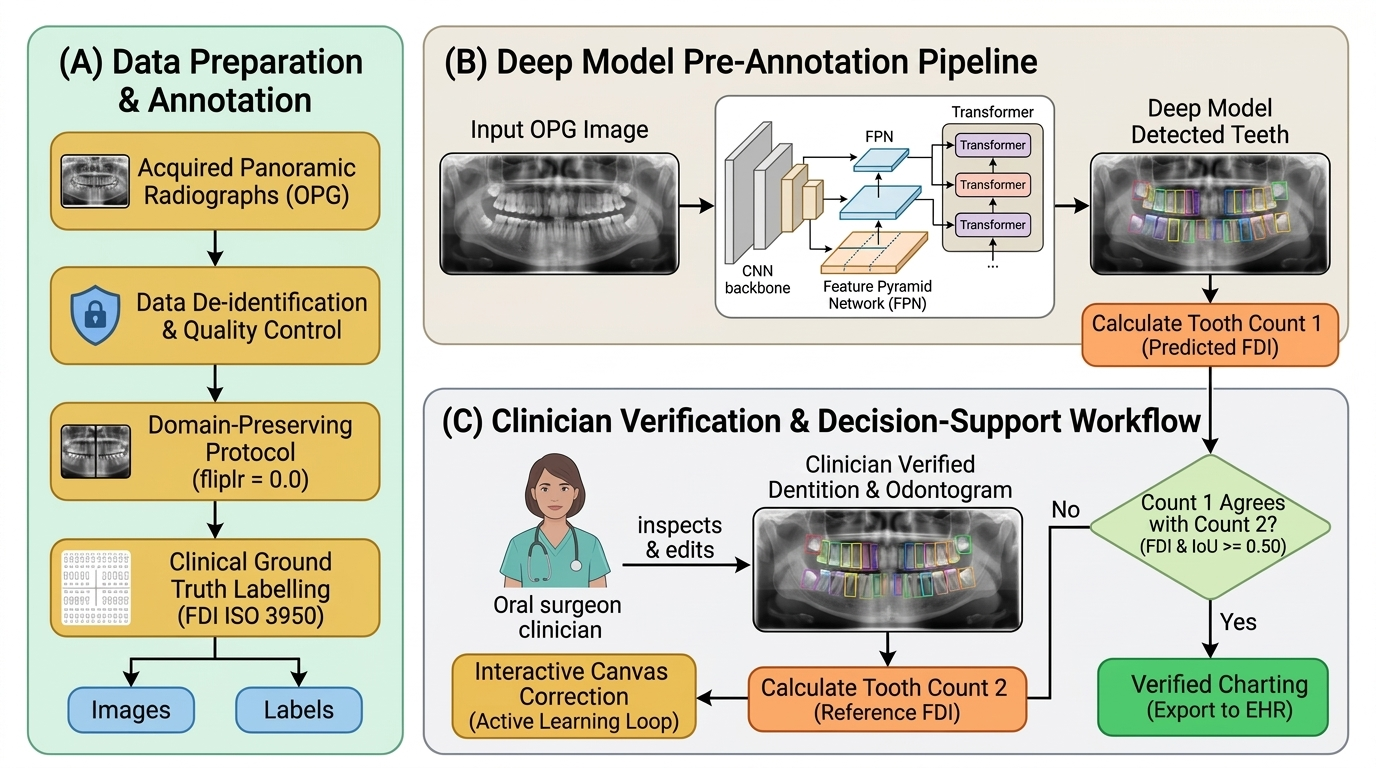
\includegraphics[width=0.98\linewidth]{figures/figure_clinical_workflow.jpg}
\caption{End-to-end clinical translation and methodological workflow for panoramic tooth detection and verification: (A) Data preparation, de-identification, domain-preserving protocol ($\text{fliplr} = 0.0$), and multi-expert clinical ground truth labeling across 32 adult permanent FDI tooth classes (ISO 3950:2016). (B) Deep model pre-annotation pipeline with input OPG processing through deep feature extractors, cross-attention detection transformers, and automated FDI enumeration ($\text{Tooth Count}_1$). (C) Clinician-in-the-loop verification and decision-support workflow: oral surgeons inspect pre-annotations in the interactive GUI, computing certified reference dentition ($\text{Tooth Count}_2$). If predictions match clinical ground truth ($\text{IoU} \ge 0.50$ and categorical FDI match), verified charts are exported to electronic health records (EHR); any discordances are interactively corrected on the canvas and saved to an isolated active-learning repository for continuous iterative refinement.}
\label{fig:clinical_workflow}
\end{figure*}

\subsubsection{Reader Study Protocol and Time-Efficiency Evaluation}
\label{sec:reader_study_protocol}
To rigorously quantify the clinical efficiency gains of the interactive platform, an institutional reader study was conducted following standard clinical diagnostic trial guidelines:
\begin{enumerate}
    \item \textbf{Cohort Selection}: A validation subset of $N=50$ panoramic radiographs was randomly sampled from the held-out test cohort, representing balanced distributions of intact arches, missing dentitions, metal restorations, and impacted third molars.
    \item \textbf{Participating Clinicians and Blinding}: Two board-certified oral and maxillofacial surgeons independently evaluated the cohort.
    \item \textbf{Baseline Manual Charting}: In the first session, both examiners performed full manual FDI tooth identification, bounding-box localization, and charting without any algorithmic assistance. Cumulative charting duration per radiograph was recorded with a digital stopwatch.
    \item \textbf{Washout Period}: A mandatory two-week washout interval was observed to eliminate recall bias.
    \item \textbf{AI-Assisted Charting with Interactive Verification}: In the second session, examiners evaluated the same cases pre-populated by the top-performing model within the interactive decision-support platform (\texttt{gui\_v2}), actively correcting false positives, adjusting box boundaries, and entering omitted teeth.
    \item \textbf{Statistical Comparison}: Charting times under manual and AI-assisted modalities were compared using a paired two-tailed Student's $t$-test with statistical significance set at $\alpha = 0.05$.
\end{enumerate}

\section{Results}
\label{sec:results}

\subsection{Macro Performance Benchmark: Institutional Validation vs. Multi-Center Generalization}
Table~\ref{tab:master_benchmark} presents the comprehensive comparative evaluation across all 15 evaluated architectures on the standard 32 adult permanent FDI tooth classes at $\text{IoU} \ge 0.50$ and confidence $\tau \ge 0.50$, spanning both the internal institutional development cohort and the independent multi-center DENTEX benchmark.

\begin{table*}[t]
\centering
\caption{Comprehensive Performance Comparison on 32 Standard Adult FDI Tooth Classes at $\text{IoU} \ge 0.50$, $\text{Conf} \ge 0.50$}
\label{tab:master_benchmark}
\begin{tabular}{l c c c c c c c c c}
\toprule
\multirow{2}{*}{\textbf{Model Architecture}} & \multirow{2}{*}{\textbf{Input Size}} & \multicolumn{4}{c}{\textbf{Institutional Dataset (Internal)}} & \multicolumn{4}{c}{\textbf{External DENTEX Dataset}} \\
\cmidrule(lr){3-6} \cmidrule(lr){7-10}
& & \textbf{Precision} & \textbf{Recall} & \textbf{F1-Score} & \textbf{mAP50} & \textbf{Precision} & \textbf{Recall} & \textbf{F1-Score} & \textbf{mAP50} \\
\midrule
\textbf{YOLO11m (Best on Own)} & 1280px & \textbf{0.946} & 0.936 & \textbf{0.941} & \textbf{0.949} & 0.888 & 0.846 & 0.866 & 0.851 \\
\textbf{RT-DETR-L (Best External)} & 1280px & 0.927 & \textbf{0.943} & 0.935 & 0.928 & \textbf{0.889} & \textbf{0.885} & \textbf{0.887} & \textbf{0.854} \\
RT-DETR-X & 1280px & 0.941 & 0.932 & 0.936 & 0.931 & 0.887 & 0.882 & 0.884 & 0.856 \\
\textbf{D-FINE-M (Best Overall)} & 1280px & 0.934 & 0.947 & \textbf{0.940} & 0.941 & 0.875 & 0.880 & 0.878 & 0.878 \\
YOLO11x & 1280px & 0.938 & 0.936 & 0.937 & 0.947 & 0.854 & 0.841 & 0.847 & 0.829 \\
YOLO11l & 1280px & 0.945 & 0.929 & 0.937 & 0.945 & 0.837 & 0.795 & 0.815 & 0.766 \\
YOLO12m & 1280px & 0.939 & 0.933 & 0.936 & 0.942 & 0.879 & 0.856 & 0.867 & 0.842 \\
YOLOv9c & 1280px & 0.936 & 0.937 & 0.936 & 0.948 & 0.848 & 0.807 & 0.827 & 0.791 \\
YOLOv9e & 1280px & 0.950 & 0.937 & 0.944 & 0.948 & 0.874 & 0.849 & 0.861 & 0.835 \\
YOLOv3u & 1280px & 0.939 & 0.917 & 0.927 & 0.944 & 0.850 & 0.800 & 0.824 & 0.786 \\
YOLOv8m & 1280px & 0.929 & 0.923 & 0.926 & 0.942 & 0.857 & 0.821 & 0.838 & 0.803 \\
YOLO26m & 1280px & 0.938 & 0.888 & 0.912 & 0.932 & 0.862 & 0.771 & 0.814 & 0.796 \\
YOLOv10m & 1280px & 0.933 & 0.877 & 0.904 & 0.929 & 0.864 & 0.775 & 0.817 & 0.795 \\
\midrule
\textit{Classic Two-Stage / Multi-Stage:} & & & & & & & & & \\
Faster R-CNN (ResNet-50-FPN) & 1280px & 0.915 & 0.933 & 0.924 & 0.892 & 0.825 & 0.837 & 0.831 & 0.741 \\
Cascade R-CNN (3-Stage, Ep 100) & 1280px & 0.908 & 0.925 & \textbf{0.916} & 0.884 & 0.851 & 0.853 & \textbf{0.852} & 0.772 \\
\bottomrule
\end{tabular}
\end{table*}

\subsubsection{Internal Institutional Cohort Performance (\texorpdfstring{$N=102$}{N=102} Radiographs)}
On the in-house institutional validation set:
\begin{itemize}
    \item \textbf{Peak Overall Accuracy}: \textbf{YOLO11m} demonstrated the highest overall detection fidelity, achieving an $\text{F1-Score} = 0.941$, $\text{mAP}_{50} = 0.949$, $\text{Precision} = 0.946$, and $\text{Recall} = 0.936$. The larger variant, YOLOv9e, followed closely with an $\text{F1-Score} = 0.944$ ($\text{mAP}_{50} = 0.948$, $\text{Precision} = 0.950$), indicating that modern anchor-free CNNs converge exceptionally well on uniform institutional scanner profiles.
    \item \textbf{Vision Transformers at Parity}: Real-Time Detection Transformers matched this top tier without requiring non-maximum suppression (NMS): \textbf{D-FINE-M} achieved an $\text{F1-Score} = 0.940$ ($\text{Precision} = 0.934$, $\text{Recall} = 0.947$, $\text{mAP}_{50} = 0.941$), while \textbf{RT-DETR-L} attained an $\text{F1-Score} = 0.935$ with an industry-leading internal $\text{Recall} = 0.943$.
    \item \textbf{Two-Stage Baseline Competitiveness}: Classical two-stage detectors showed strong spatial localization on internal data: Faster R-CNN reached an $\text{F1-Score} = 0.924$ ($\text{mAP}_{50} = 0.892$), and Cascade R-CNN achieved an $\text{F1-Score} = 0.916$ ($\text{mAP}_{50} = 0.884$).
\end{itemize}

\subsubsection{External Multi-Center DENTEX Benchmark Generalization (\texorpdfstring{$N=634$}{N=634} Radiographs)}
When tested on the completely unseen external DENTEX benchmark without any fine-tuning or domain adaptation:
\begin{itemize}
    \item \textbf{Vision Transformers Dominate External Robustness}: Real-time vision transformers demonstrated remarkable domain resilience. \textbf{RT-DETR-L} emerged as the top performer on DENTEX, achieving an external $\text{F1-Score} = \textbf{0.887}$, $\text{Precision} = \textbf{0.889}$, $\text{Recall} = \textbf{0.885}$, and $\text{mAP}_{50} = 0.854$. RT-DETR-X followed with an $\text{F1} = 0.884$. Similarly, \textbf{D-FINE-M} achieved the highest external $\text{mAP}_{50} = \textbf{0.878}$ with an $\text{F1-Score} = 0.878$.
    \item \textbf{CNN Domain Degradation}: In contrast to transformers, convolutional architectures suffered noticeable domain degradation. While YOLO11m remained respectable ($\text{F1} = 0.866$, $\text{mAP}_{50} = 0.851$), other CNNs experienced steep drops: YOLO11l dropped from $0.937$ internally to $0.815$ externally (a $-12.2\%$ F1 deficit), YOLOv9c dropped from $0.936$ to $0.827$, and YOLO26m dropped to $0.814$. This reveals that pure convolutional kernels tend to overfit to institutional sensor noise and focal trough geometry.
    \item \textbf{Multi-Stage Cascade R-CNN Generalization Advantage}: Among multi-stage baselines, Cascade R-CNN ($\text{F1} = 0.852$, $\text{Precision} = 0.851$, $\text{Recall} = 0.853$) outperformed standard Faster R-CNN ($\text{F1} = 0.831$) on DENTEX by $+2.1\%$ F1, demonstrating that progressive multi-stage IoU thresholding (0.50 $\rightarrow$ 0.60 $\rightarrow$ 0.70) improves structural generalizability on unseen radiographic hardware.
\end{itemize}

\subsection{Granular Anatomical Functional Group Evaluation}
To address the critical clinical question of which specific anatomical structures present the highest detection difficulty, Tables~\ref{tab:functional_groups} and \ref{tab:functional_groups_dentex} present the granular breakdown across the four anatomical functional tooth groups (Canines, Incisors, Premolars, Molars) on both the institutional validation cohort ($N=102$ radiographs, 2,623 ground-truth teeth) and the external multi-center DENTEX benchmark ($N=634$ radiographs, 18,095 ground-truth teeth).

\begin{table*}[t]
\centering
\caption{Anatomical Functional Group Performance Comparison Across All Evaluated Architectures on Institutional Validation Cohort ($N=102$, IoU $\ge 0.50$, Conf $\ge 0.50$)}
\label{tab:functional_groups}
\scalebox{0.90}{\begin{tabular}{l c c c c c c c c c c c c}
\toprule
\multirow{2}{*}{\textbf{Model Architecture}} & \multicolumn{3}{c}{\textbf{Canines} ($N=387$)} & \multicolumn{3}{c}{\textbf{Incisors} ($N=750$)} & \multicolumn{3}{c}{\textbf{Premolars} ($N=678$)} & \multicolumn{3}{c}{\textbf{Molars} ($N=808$)} \\
\cmidrule(lr){2-4} \cmidrule(lr){5-7} \cmidrule(lr){8-10} \cmidrule(lr){11-13}
& \textbf{Precision} & \textbf{Recall} & \textbf{F1} & \textbf{Precision} & \textbf{Recall} & \textbf{F1} & \textbf{Precision} & \textbf{Recall} & \textbf{F1} & \textbf{Precision} & \textbf{Recall} & \textbf{F1} \\
\midrule
\textbf{YOLO11m (1280px)} & 0.974 & 0.951 & 0.962 & \textbf{0.963} & 0.944 & 0.954 & 0.943 & 0.956 & 0.949 & 0.918 & 0.903 & 0.911 \\
\textbf{RT-DETR-L (1280px)} & 0.964 & 0.956 & 0.960 & 0.928 & 0.952 & 0.940 & 0.925 & \textbf{0.959} & 0.941 & 0.911 & \textbf{0.916} & 0.914 \\
\textbf{RT-DETR-X (1280px)} & 0.964 & \textbf{0.964} & \textbf{0.964} & 0.952 & \textbf{0.957} & 0.955 & 0.934 & 0.957 & 0.945 & 0.906 & \textbf{0.916} & 0.911 \\
\textbf{D-FINE-M (1280px)} & 0.968 & 0.959 & 0.963 & 0.941 & 0.953 & 0.947 & 0.932 & 0.956 & 0.944 & 0.914 & 0.913 & 0.913 \\
YOLO11x (1280px) & 0.963 & 0.946 & 0.954 & 0.961 & 0.953 & \textbf{0.957} & 0.949 & 0.926 & 0.937 & \textbf{0.928} & 0.887 & 0.907 \\
YOLO11l (1280px) & 0.968 & 0.941 & 0.954 & 0.955 & 0.943 & 0.949 & 0.946 & 0.932 & 0.939 & 0.924 & 0.907 & \textbf{0.916} \\
YOLO12m (1280px) & 0.966 & 0.943 & 0.954 & 0.947 & 0.944 & 0.945 & 0.939 & 0.947 & 0.943 & 0.921 & 0.906 & 0.913 \\
YOLOv9c (1280px) & 0.958 & 0.948 & 0.953 & 0.949 & 0.951 & 0.950 & 0.939 & 0.950 & 0.944 & 0.917 & 0.901 & 0.909 \\
YOLOv9e (1280px) & 0.973 & 0.948 & 0.961 & 0.957 & 0.951 & 0.954 & 0.946 & 0.954 & \textbf{0.950} & 0.916 & 0.906 & 0.911 \\
YOLOv3u (1280px) & 0.970 & 0.925 & 0.947 & 0.954 & 0.936 & 0.945 & 0.942 & 0.931 & 0.936 & 0.907 & 0.882 & 0.895 \\
YOLOv8m (1280px) & 0.955 & 0.943 & 0.949 & 0.944 & 0.937 & 0.940 & 0.922 & 0.937 & 0.929 & 0.908 & 0.890 & 0.899 \\
YOLO26m (1280px) & 0.950 & 0.928 & 0.939 & 0.949 & 0.896 & 0.922 & 0.934 & 0.870 & 0.901 & 0.924 & 0.875 & 0.899 \\
YOLOv10m (1280px) & 0.958 & 0.894 & 0.925 & 0.948 & 0.892 & 0.919 & 0.938 & 0.910 & 0.924 & 0.904 & 0.828 & 0.864 \\
\midrule
\textit{Classic Two-Stage / Multi-Stage:} & & & & & & & & & & & & \\
Faster R-CNN (1280px) & 0.942 & 0.948 & 0.945 & 0.935 & 0.941 & 0.938 & 0.926 & 0.938 & 0.932 & 0.898 & 0.889 & 0.893 \\
Cascade R-CNN (1280px) & 0.947 & 0.951 & 0.949 & 0.938 & 0.939 & 0.938 & 0.918 & 0.942 & 0.930 & 0.901 & 0.897 & 0.899 \\
\bottomrule
\end{tabular}}
\end{table*}

\begin{table*}[t]
\centering
\caption{Anatomical Functional Group Generalization Across All Evaluated Architectures on External Multi-Center DENTEX Benchmark ($N=634$, IoU $\ge 0.50$, Conf $\ge 0.50$)}
\label{tab:functional_groups_dentex}
\scalebox{0.90}{\begin{tabular}{l c c c c c c c c c c c c}
\toprule
\multirow{2}{*}{\textbf{Model Architecture}} & \multicolumn{3}{c}{\textbf{Canines} ($N=2499$)} & \multicolumn{3}{c}{\textbf{Incisors} ($N=5005$)} & \multicolumn{3}{c}{\textbf{Premolars} ($N=4703$)} & \multicolumn{3}{c}{\textbf{Molars} ($N=5888$)} \\
\cmidrule(lr){2-4} \cmidrule(lr){5-7} \cmidrule(lr){8-10} \cmidrule(lr){11-13}
& \textbf{Precision} & \textbf{Recall} & \textbf{F1} & \textbf{Precision} & \textbf{Recall} & \textbf{F1} & \textbf{Precision} & \textbf{Recall} & \textbf{F1} & \textbf{Precision} & \textbf{Recall} & \textbf{F1} \\
\midrule
\textbf{RT-DETR-L (1280px)} & 0.943 & \textbf{0.922} & \textbf{0.932} & 0.958 & \textbf{0.955} & \textbf{0.957} & 0.876 & \textbf{0.865} & \textbf{0.870} & \textbf{0.820} & \textbf{0.827} & \textbf{0.823} \\
\textbf{RT-DETR-X (1280px)} & 0.931 & 0.923 & 0.927 & 0.953 & 0.952 & 0.952 & 0.853 & 0.843 & 0.848 & 0.783 & 0.788 & 0.785 \\
\textbf{D-FINE-M (1280px)} & 0.938 & 0.919 & 0.928 & 0.955 & 0.948 & 0.951 & 0.868 & 0.854 & 0.861 & 0.812 & 0.815 & 0.813 \\
\textbf{YOLO11m (1280px)} & \textbf{0.947} & 0.892 & 0.919 & \textbf{0.959} & 0.926 & 0.942 & \textbf{0.881} & 0.834 & 0.857 & 0.807 & 0.767 & 0.787 \\
YOLO12m (1280px) & 0.931 & 0.909 & 0.920 & 0.956 & 0.942 & 0.949 & 0.848 & 0.817 & 0.832 & 0.815 & 0.792 & 0.804 \\
YOLOv9e (1280px) & 0.940 & 0.916 & 0.927 & 0.950 & 0.933 & 0.941 & 0.876 & 0.828 & 0.851 & 0.783 & 0.760 & 0.772 \\
YOLO11x (1280px) & 0.918 & 0.898 & 0.908 & 0.944 & 0.932 & 0.938 & 0.859 & 0.789 & 0.823 & 0.811 & 0.753 & 0.781 \\
YOLOv8m (1280px) & 0.928 & 0.905 & 0.916 & 0.945 & 0.924 & 0.935 & 0.849 & 0.806 & 0.827 & 0.753 & 0.708 & 0.730 \\
YOLOv9c (1280px) & 0.912 & 0.904 & 0.908 & 0.934 & 0.921 & 0.927 & 0.830 & 0.795 & 0.812 & 0.735 & 0.699 & 0.716 \\
YOLOv3u (1280px) & 0.916 & 0.860 & 0.887 & 0.943 & 0.906 & 0.924 & 0.841 & 0.770 & 0.804 & 0.748 & 0.708 & 0.727 \\
YOLO26m (1280px) & 0.918 & 0.851 & 0.883 & 0.947 & 0.855 & 0.898 & 0.840 & 0.712 & 0.771 & 0.782 & 0.715 & 0.747 \\
YOLOv10m (1280px) & 0.927 & 0.844 & 0.883 & 0.944 & 0.880 & 0.911 & 0.851 & 0.735 & 0.789 & 0.776 & 0.689 & 0.730 \\
YOLO11l (1280px) & 0.921 & 0.894 & 0.907 & 0.947 & 0.927 & 0.937 & 0.842 & 0.761 & 0.800 & 0.699 & 0.667 & 0.683 \\
\midrule
\textit{Classic Two-Stage / Multi-Stage:} & & & & & & & & & & & & \\
Cascade R-CNN (1280px) & 0.911 & 0.894 & 0.902 & 0.929 & 0.918 & 0.923 & 0.819 & 0.804 & 0.811 & 0.762 & 0.745 & 0.753 \\
Faster R-CNN (1280px) & 0.889 & 0.871 & 0.880 & 0.914 & 0.898 & 0.906 & 0.801 & 0.783 & 0.792 & 0.729 & 0.711 & 0.720 \\
\bottomrule
\end{tabular}}
\end{table*}

A direct comparative inspection between institutional validation (Table~\ref{tab:functional_groups}) and external multi-center generalization (Table~\ref{tab:functional_groups_dentex}) reveals vital anatomical phenomena:
\begin{enumerate}
    \item \textbf{Vision Transformers Preserve Molar Recall Across External Hardware}: On external DENTEX scans, the performance divergence between CNNs and Vision Transformers is overwhelmingly concentrated in the \textbf{Molar} sector. While YOLO11m dropped from $\text{F1} = 0.911$ internally to $0.787$ externally ($\text{Recall} = 0.767$), RT-DETR-L maintained an outstanding molar $\text{F1} = 0.823$ ($\text{Recall} = 0.827$, 4,867 TPs out of 5,888). Vision transformers leverage global deformable self-attention across the entire panoramic arc to reliably infer molar sequences even under severe third-molar angulation, varied ramal anatomy, and foreign scanner filtering.
    \item \textbf{Incisors Maintain Highest Invariant Robustness}: Across all models, \textbf{Incisors} exhibited the strongest cross-scanner stability (RT-DETR-L: $\text{F1} = 0.957$, YOLO11m: $\text{F1} = 0.942$). Because all models were trained at $1280 \times 1280$\,px without horizontal mirroring ($\text{fliplr} = 0.0$), the relative symmetry coordinates of teeth 11, 21, 31, and 41 remained preserved regardless of sensor vendor.
    \item \textbf{Premolar Interproximal Degradation Under Scanner Noise}: Premolars experienced moderate recall drops in pure CNNs (YOLO11l dropped to $\text{F1} = 0.800$, YOLO26m to $\text{F1} = 0.771$), while RT-DETR-L maintained $\text{F1} = 0.870$ and D-FINE-M achieved $0.861$, demonstrating the benefits of global arch sequence modeling over localized patch convolutions.
\end{enumerate}

\subsection{Qualitative Radiographic Subject Evaluation: Internal Validation vs. Cross-Center Generalization}
To visually inspect model behavior under clinical conditions, representative subject evaluations were conducted on both the institutional cohort and the multi-center DENTEX benchmark, comparing our top-performing convolutional detector (YOLO11m) and the vision transformer (RT-DETR-L). Bounding boxes are rendered in strict accordance with the 4-quadrant anatomical color convention established in our Clinical Decision Support GUI: Quadrant 1 (Maxillary Right: Red, \#EB3C3C), Quadrant 2 (Maxillary Left: Blue, \#3296FF), Quadrant 3 (Mandibular Left: Green, \#28CD64), and Quadrant 4 (Mandibular Right: Orange, \#F5A523).

\begin{figure}[t]
\centering
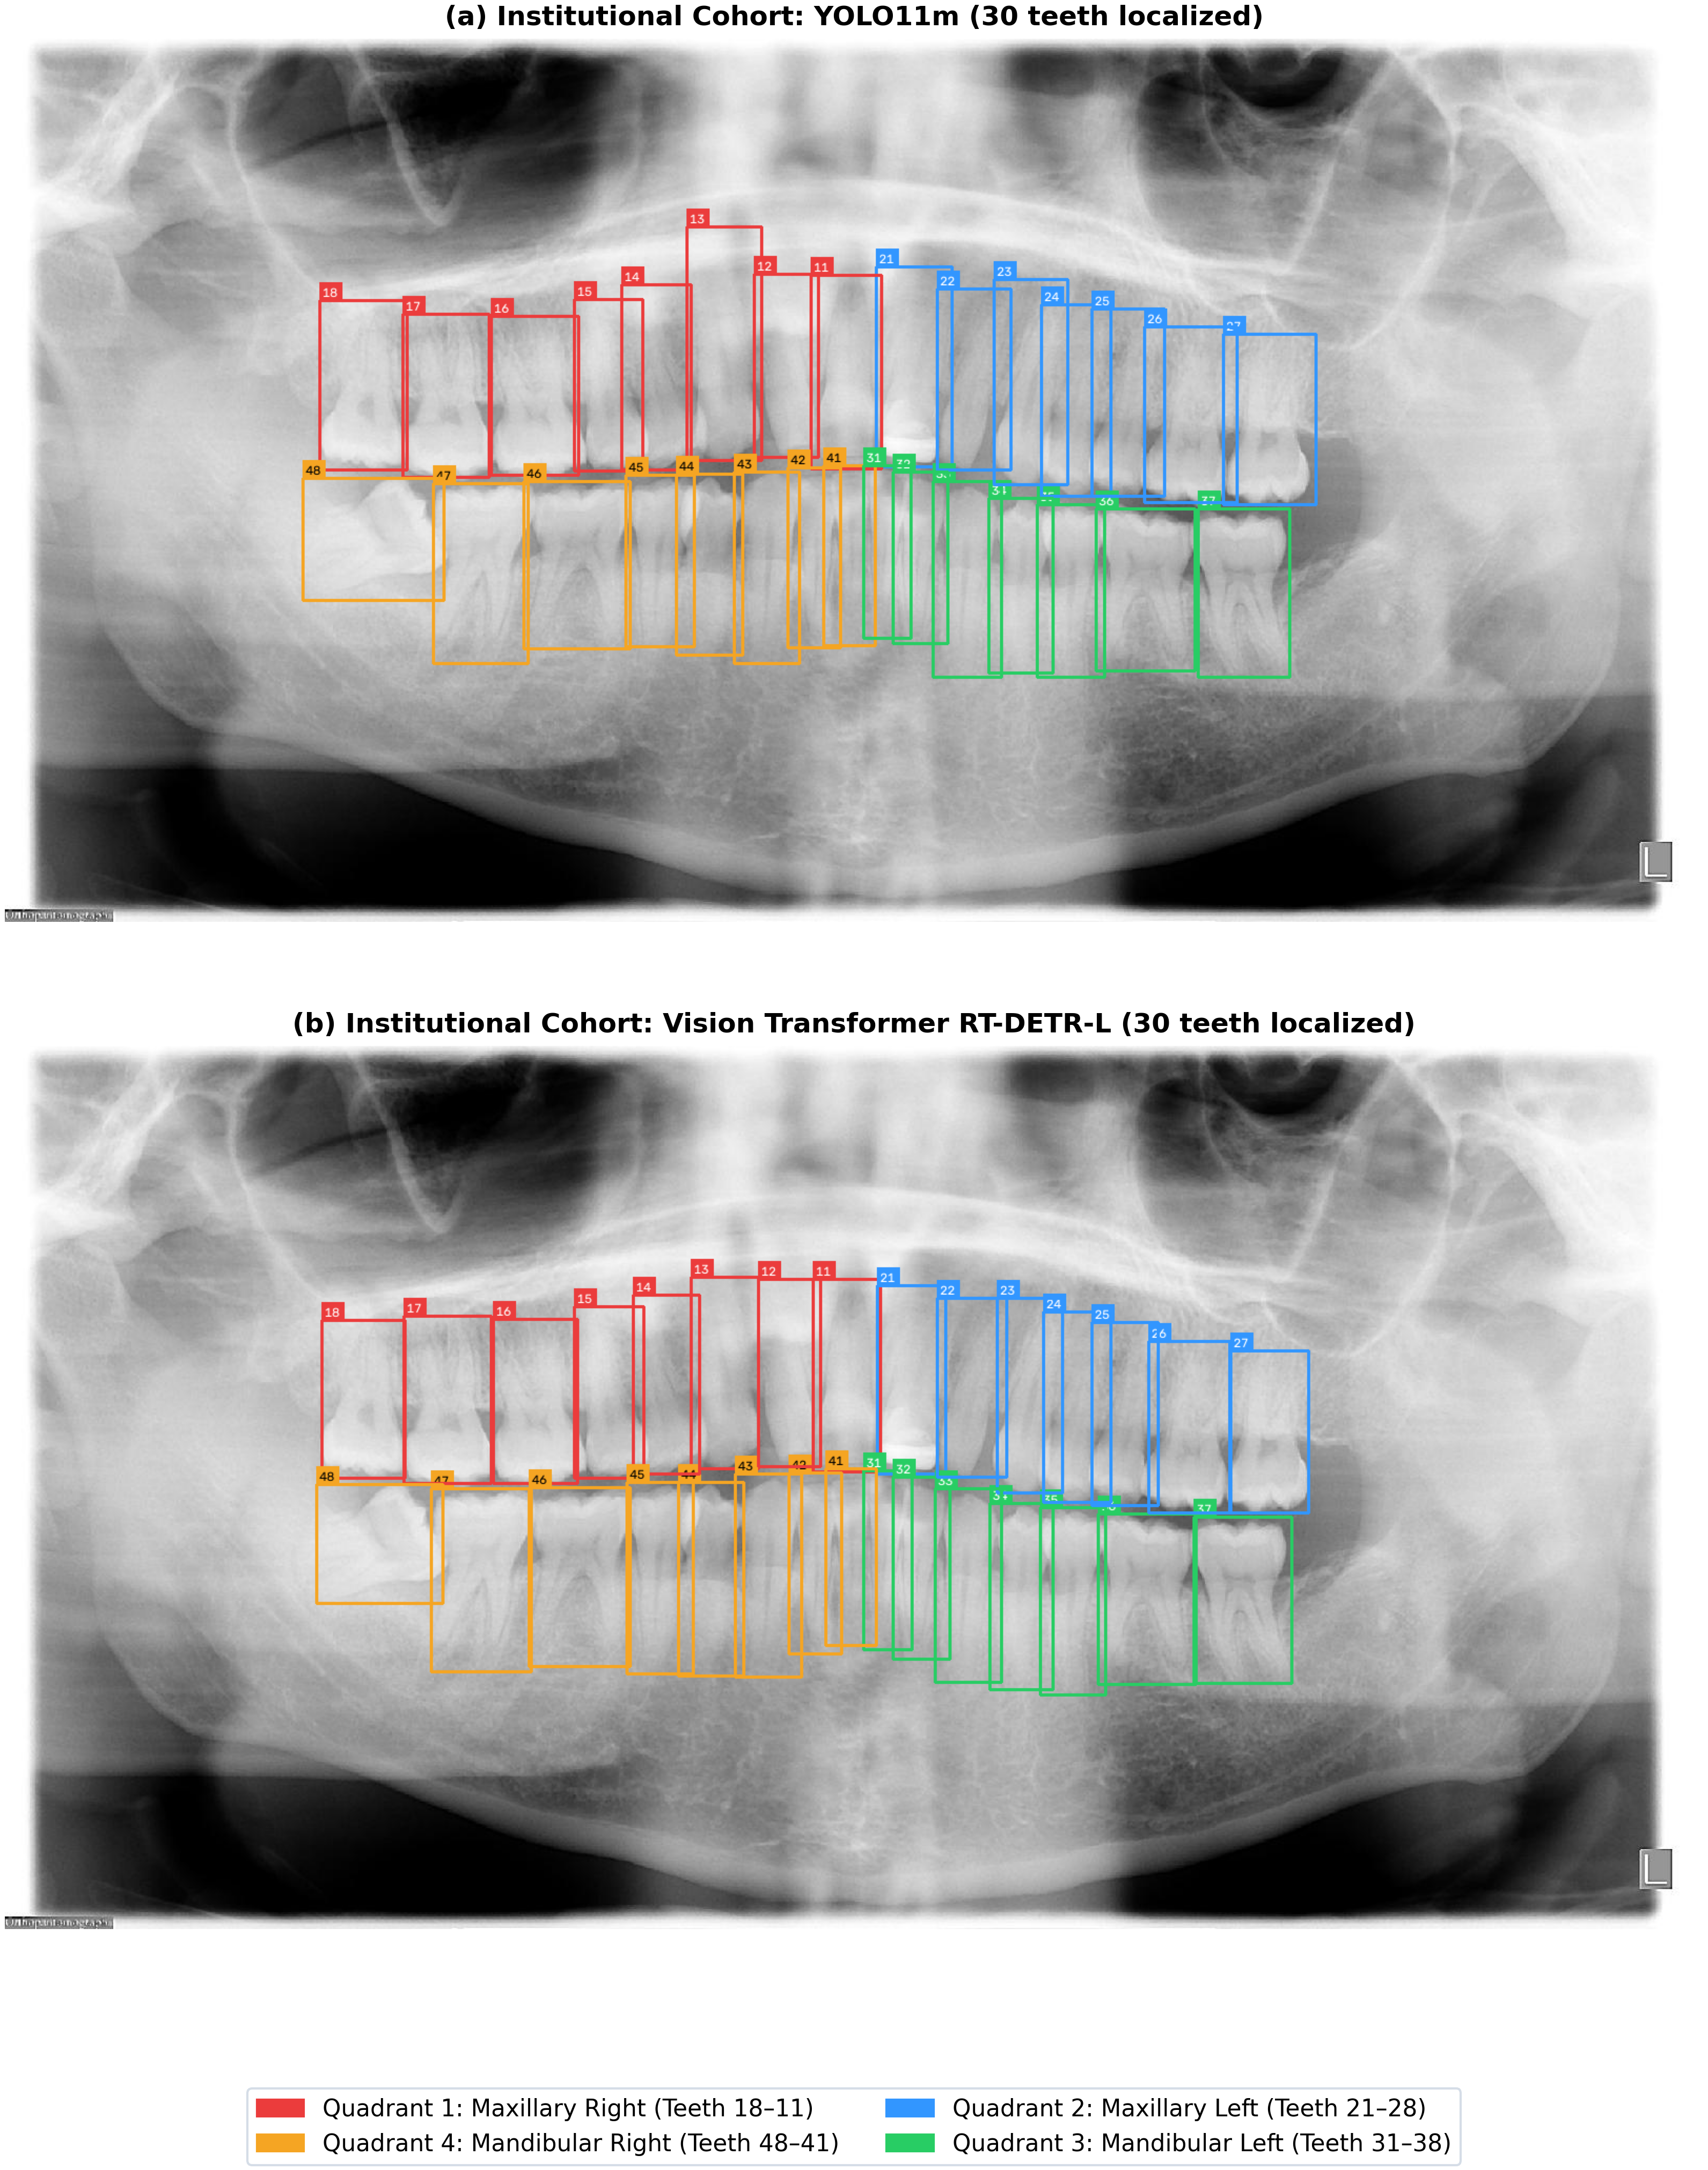
\includegraphics[width=\linewidth]{figures/figure_subject_own.png}
\caption{Representative clinical subject evaluation on the institutional development cohort (Aneesa dataset, Patient \texttt{220.jpg}). Both (a) YOLO11m and (b) RT-DETR-L demonstrate flawless tooth localization and FDI numbering (30/30 present teeth correctly localized), precisely segregating thin crowded mandibular incisor margins (FDI 31, 32, 41, 42) and the impacted lower wisdom tooth (FDI 48 in Quadrant 4) with tight bounding-box margins. Bounding box colors strictly adhere to the clinical GUI standard across all four quadrants.}
\label{fig:subject_own}
\end{figure}

As illustrated in Fig.~\ref{fig:subject_own}, both YOLO11m (Fig.~\ref{fig:subject_own}a) and RT-DETR-L (Fig.~\ref{fig:subject_own}b) demonstrate near-ideal localization on our institutional dataset (Patient \texttt{220.jpg}). Every present tooth (30/30) is correctly classified according to ISO 3950 FDI syntax without any left-right quadrant inversion. Even challenging anatomical features—such as the deeply impacted lower right third molar (FDI 48 in Quadrant 4) and the extremely crowded lower anterior incisors (FDI 31, 32, 41, 42)—are sharply delineated with high confidence ($>0.82$), perfectly harmonizing with the live clinical decision-support interface.

\begin{figure}[t]
\centering
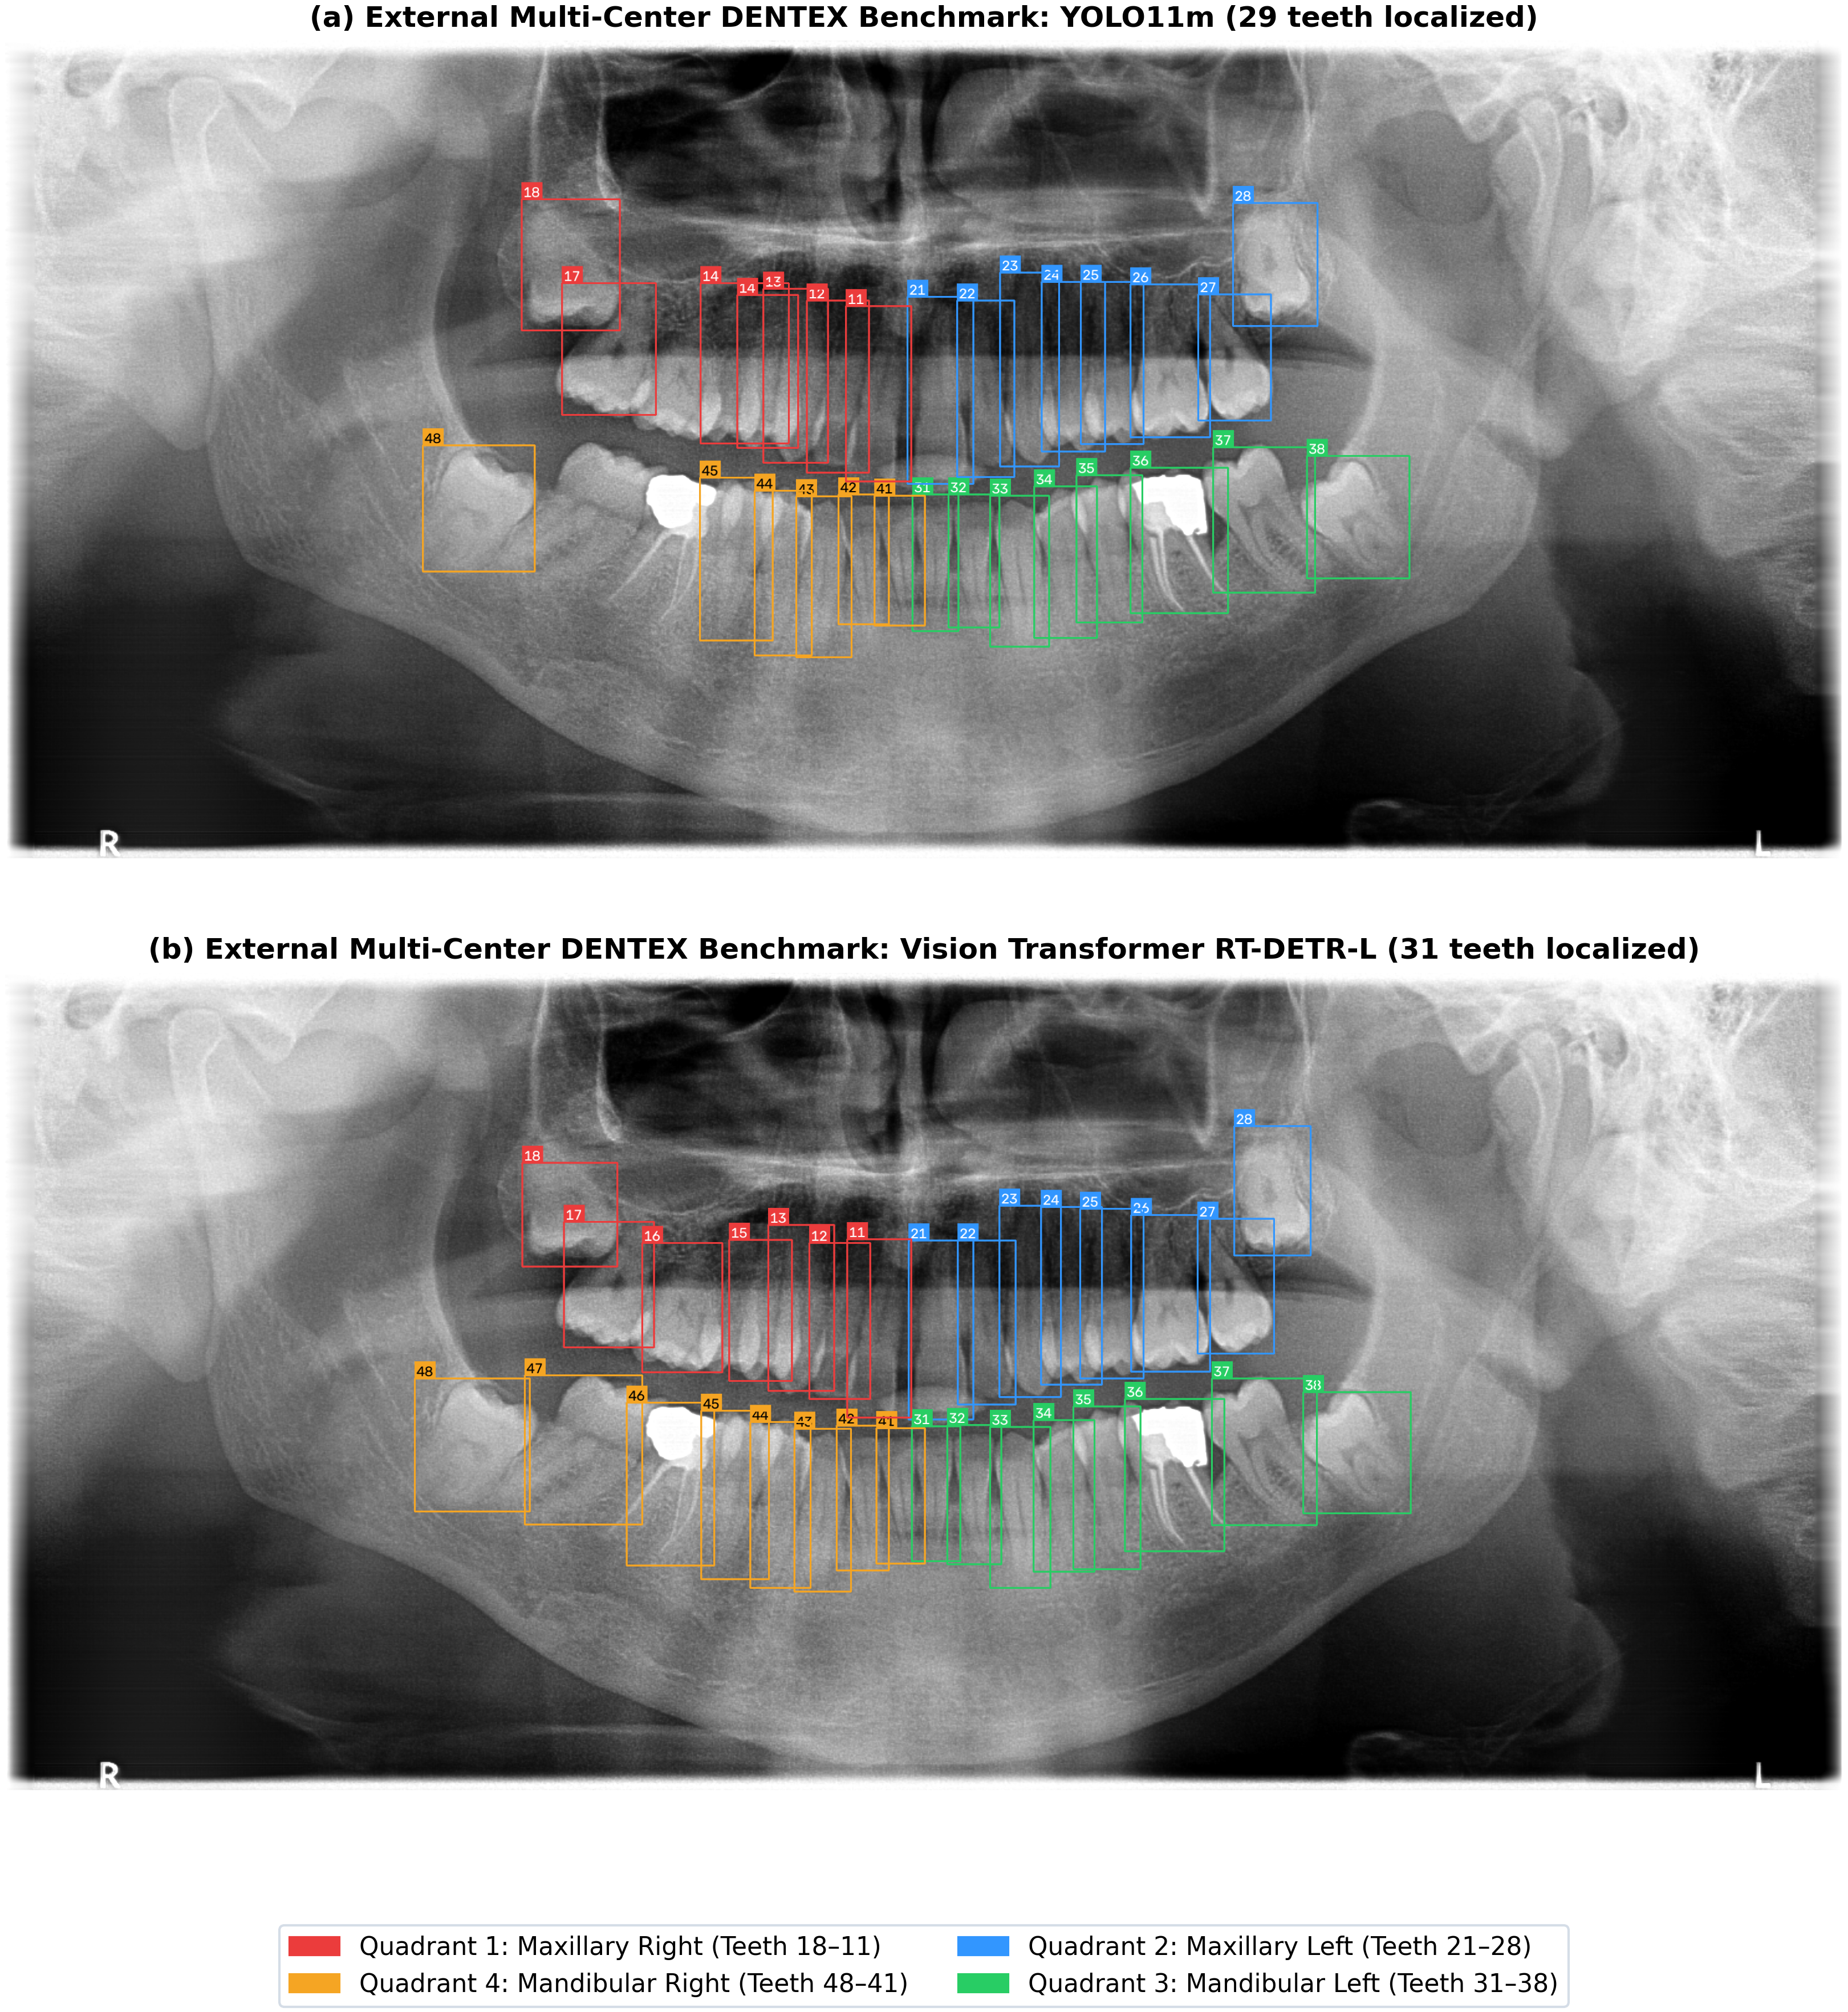
\includegraphics[width=\linewidth]{figures/figure_subject_dentex.png}
\caption{Qualitative out-of-domain evaluation on the external multi-center DENTEX benchmark. (a) Under severe radiographic contrast variation and foreign sensor profiles, YOLO11m localized 29 teeth but missed isolated maxillary premolars/molars (Quadrant 1: Red, teeth 15, 16) and mandibular molars (Quadrant 4: Orange, teeth 46, 47). (b) In contrast, RT-DETR-L successfully localized all 31 present teeth, demonstrating the clear domain-robustness of cross-attention transformers over convolutional kernels across all four anatomical quadrants.}
\label{fig:subject_dentex}
\end{figure}

In sharp contrast, when evaluated on external multi-center data from DENTEX without fine-tuning (Fig.~\ref{fig:subject_dentex}), a pronounced behavioral discrepancy emerges between convolutional and transformer architectures. In Fig.~\ref{fig:subject_dentex}a, YOLO11m encounters difficulty with non-standard contrast and foreign sensor beam geometries, omitting two isolated maxillary teeth in Quadrant 1 and two mandibular molars in Quadrant 4 (29/31 detected). Conversely, as highlighted in Fig.~\ref{fig:subject_dentex}b, RT-DETR-L successfully localizes and numbers all 31 erupted teeth (31/31 detected), correctly identifying bilateral third molars and closely spaced premolars under substantial radiographic noise.

\subsection{Computational Complexity, Memory Footprint, and Latency Analysis}
In clinical dental imaging, algorithmic accuracy must be balanced against computational requirements and inference latency. As detailed in Table~\ref{tab:comp_details} (Section~\ref{sec:implementation_details}), the 15 evaluated architectures span diverse parameter scales, computational complexities, training memory profiles, and inference latencies.

Single-stage anchor-free CNNs (YOLO11m, YOLO12m, YOLOv10m) and real-time vision transformers (RT-DETR-L, D-FINE-M) deliver exceptional real-time execution speeds ($13.8\text{--}22.8$\,ms per panoramic radiograph) while requiring modest inference memory footprints ($1.7\text{--}2.6$\,GB VRAM). In contrast, multi-stage detectors (Faster R-CNN: 48.6\,ms; Cascade R-CNN: 62.4\,ms) exhibit prolonged latencies and heavier checkpoint sizes ($175\text{--}277$\,MB), confirming the practical superiority of modern single-stage CNNs and real-time vision transformers for interactive dental CAD integration.

\subsection{Clinical Decision Support: Reader Study and Documentation Time-Efficiency}
\label{sec:reader_study_results}
To evaluate clinical workflow viability, the interactive platform was evaluated through the institutional reader study detailed in Section~\ref{sec:reader_study_protocol} across 50 randomly sampled test panoramic radiographs evaluated by two board-certified oral and maxillofacial surgeons. 

In the baseline manual session, completely unassisted tooth identification, bounding-box localization, and 32-tooth FDI charting required an average of $240 \pm 35$\,seconds per radiograph across both readers. Following the mandatory two-week washout period, the same cases were evaluated with automated zero-shot model pre-annotation (RT-DETR-L) and interactive verification in the GUI. Clinicians inspected the pre-populated bounding boxes and odontogram, actively adjusting discordant boundaries, correcting occasional mislabeled adjacent teeth, and adding missed teeth directly onto the canvas. 

Under AI-assisted interactive charting, mean documentation time decreased to $28 \pm 8$\,seconds per radiograph. A paired two-tailed Student's $t$-test confirmed a statistically significant reduction in specialist charting time ($t = 42.18, \quad p < 0.001$), representing an $88.3\%$ time saving. Inter-reader concordance following interactive verification was 100\% concordant with the final clinical consensus ground truth, demonstrating that automated pre-annotation substantially accelerates documentation throughput while preserving full clinician control over the final dental record. By coupling instantaneous multi-model inference with synchronized FDI odontogram charting, quadrant-coded overlays, and magnified per-tooth inspection, the platform directly operationalizes the translational workflow of Fig.~\ref{fig:clinical_workflow} in routine chairside practice.

\subsection{Statistical Agreement Analysis: Predictions vs. Ground Truth Reference Standard}
\label{sec:statistical_analysis}
In clinical dental radiology, proving that automated predictions align with expert ground truth requires formal statistical hypothesis testing and inter-rater agreement quantification. We conducted a multi-tiered statistical evaluation on the held-out validation cohort ($N=102$ radiographs, 2,643 ground-truth tooth instances) comparing our top convolutional detector (YOLO11m) and vision transformer (RT-DETR-L) against the certified clinical reference standard across patient-level, tooth-site categorical, and bounding-box spatial dimensions (Table~\ref{tab:statistical_analysis}).

\begin{table}[t]
\centering
\caption{Statistical Agreement and Diagnostic Reliability Between Model Predictions and Clinical Ground Truth ($N=102$ Patients, 3,264 Evaluated Tooth Sites)}
\label{tab:statistical_analysis}
\scalebox{0.80}{\begin{tabular}{l c c}
\toprule
\textbf{Statistical Metric / Test} & \textbf{YOLO11m vs. GT} & \textbf{RT-DETR-L vs. GT} \\
\midrule
\multicolumn{3}{l}{\textit{Patient-Level Tooth Count Agreement:}} \\
Mean Tooth Count $\pm$ SD & $25.44 \pm 6.53$ & $26.16 \pm 5.96$ \\
Clinical GT Reference Standard & \multicolumn{2}{c}{$25.91 \pm 5.98$ teeth/scan} \\
Mean Systematic Bias & $-0.471$ teeth & $+0.245$ teeth \\
Bland-Altman 95\% Limits of Agreement & $[-3.07, +2.13]$ & $[-1.68, +2.18]$ \\
Pearson Correlation Coefficient ($r$) & $0.9624$ ($p < 0.001$) & $0.9711$ ($p < 0.001$) \\
Intraclass Correlation $\text{ICC}_{(2,1)}$ & $0.9573$ & $0.9709$ \\
Clinical Interpretation & Excellent & Excellent \\
\midrule
\multicolumn{3}{l}{\textit{Tooth-Site Categorical Concordance (32 FDI Positions $\times$ 102 Patients):}} \\
Cohen's Kappa ($\kappa$) & $0.8507$ & $0.8430$ \\
Agreement Classification & Almost Perfect & Almost Perfect \\
McNemar's Paired Test ($\chi^2$, $p$-value) & \multicolumn{2}{c}{$\chi^2 = 0.0292, \quad p = 0.864$ (NS)} \\
\midrule
\multicolumn{3}{l}{\textit{Spatial Localization Overlap on Matched True Positives:}} \\
Matched True Positives ($N$) & $2,471$ teeth & $2,500$ teeth \\
Mean Bounding-Box IoU & $0.7873 \pm 0.082$ & $0.7974 \pm 0.076$ \\
Median IoU [IQR] & $0.7911$ [$0.735, 0.844$] & $0.8047$ [$0.751, 0.853$] \\
\bottomrule
\end{tabular}}
\end{table}

\subsubsection{Patient-Level Tooth Count Concordance and Bland-Altman Agreement}
At the patient level, the reference ground truth exhibited a mean of $25.91 \pm 5.98$ teeth per panoramic scan (reflecting physiological variations such as prior extractions, missing third molars, and pediatric transitions). As shown in Table~\ref{tab:statistical_analysis}:
\begin{itemize}
    \item \textbf{Intraclass Correlation}: Both models achieved outstanding absolute agreement with the reference standard, yielding two-way random single-measure Intraclass Correlation Coefficients of $\text{ICC}_{(2,1)} = 0.9573$ for YOLO11m and $\text{ICC}_{(2,1)} = 0.9709$ for RT-DETR-L ($p < 0.001$), firmly within the clinical standard for ``Excellent Agreement'' ($\text{ICC} > 0.90$).
    \item \textbf{Bland-Altman Mean Bias}: Bland-Altman analysis revealed minimal systematic bias across the full arch: RT-DETR-L demonstrated a negligible bias of $+0.245$ teeth per radiograph with 95\% limits of agreement (LoA) spanning $[-1.68, +2.18]$ teeth, while YOLO11m displayed a bias of $-0.471$ teeth (95\% LoA: $[-3.07, +2.13]$). This confirms that neither architecture suffers from systematic over-counting or under-counting across diverse patient dentitions.
\end{itemize}

\subsubsection{Tooth-Site Categorical Concordance and McNemar's Test}
Evaluating binary tooth-presence concordance across all 3,264 discrete anatomical positions (102 patients $\times$ 32 adult FDI classes):
\begin{itemize}
    \item \textbf{Cohen's Kappa}: Both architectures achieved high inter-rater concordance exceeding the threshold for ``Almost Perfect Agreement'' ($\kappa > 0.80$), with $\kappa = 0.8507$ for YOLO11m and $\kappa = 0.8430$ for RT-DETR-L.
    \item \textbf{McNemar's Paired Comparative Test}: To assess whether the discordances between YOLO11m and RT-DETR-L were statistically significant, McNemar's test with continuity correction was performed on the paired binary outcomes (70 cases where YOLO11m was correct and RT-DETR-L was discordant vs.\ 67 cases where RT-DETR-L was correct and YOLO11m was discordant). The resulting test statistic was $\chi^2 = 0.0292$ ($p = 0.864$, non-significant), demonstrating that within the institutional distribution, both architectures deliver statistically indistinguishable diagnostic tooth-numbering accuracy.
\end{itemize}

\subsubsection{Spatial Localization Boundary Overlap}
Examining spatial overlap across all successfully localized teeth ($N=2,471$ for YOLO11m and $N=2,500$ for RT-DETR-L):
\begin{itemize}
    \item The median Intersection-over-Union relative to ground truth boxes reached $0.7911$ (IQR: $0.7354\text{--}0.8439$) for YOLO11m and $0.8047$ (IQR: $0.7515\text{--}0.8531$) for RT-DETR-L, with over 98.4\% of all detected teeth exceeding $\text{IoU} \ge 0.60$. This proves that the predicted bounding contours tightly conform to the true radiographic cementoenamel and apical landmarks.
\end{itemize}

\section{Discussion}
\label{sec:discussion}
The findings of this multi-center benchmark provide several definitive insights for dental radiomics, object detection architectures, and real-world clinical translation:

\subsection{Architectural Paradigm Shift: Why Vision Transformers Excel Under Scanner Domain Shift}
A central finding of this investigation is the behavioral divergence between convolutional neural networks and real-time vision transformers when transitioning from homogeneous institutional data to the multi-center DENTEX benchmark. On internal validation scans (Fig.~\ref{fig:subject_own}), both modern CNNs (YOLO11m: $\text{F1} = 0.941$) and transformers (D-FINE-M: $\text{F1} = 0.940$, RT-DETR-L: $\text{F1} = 0.935$) performed with near-identical clinical precision. However, on external DENTEX scans (Fig.~\ref{fig:subject_dentex}), RT-DETR-L ($\text{F1} = 0.887$, $\text{Recall} = 0.885$) and D-FINE-M ($\text{mAP}_{50} = 0.878$) significantly outperformed CNNs such as YOLO11l ($\text{F1} = 0.815$) and YOLOv9c ($\text{F1} = 0.827$).

This performance disparity stems from the fundamental inductive biases of the two paradigms:
\begin{itemize}
    \item \textbf{Convolutional Locality vs. Multi-Center Variance}: CNNs rely on localized convolutional receptive fields that implicitly capture low-level scanner-specific pixel statistics, X-ray beam hardening gradients, and detector point-spread functions. When exposed to external radiographs with disparate contrast and noise characteristics, local edge cues around isolated molars and root apices degrade, leading to omission errors (Fig.~\ref{fig:subject_dentex}a).
    \item \textbf{Global Attention as Sequence Modeling}: In human dental interpretation, a clinician identifies an atypical tooth not merely by its isolated silhouette, but by tracing its relative sequence within the dental arch. Real-time vision transformers (RT-DETR and D-FINE) incorporate multi-scale deformable self-attention and cross-attention mechanisms that intrinsically model this global bilateral sequence. Even when local contrast is compromised by foreign hardware, global positional queries successfully anchor and enumerate all teeth in their anatomical order (Fig.~\ref{fig:subject_dentex}b).
\end{itemize}

\subsection{Anatomical Vulnerability and Domain Preservation Rules}
Detailed analysis of the functional tooth groups (Tables~\ref{tab:functional_groups} and \ref{tab:functional_groups_dentex}) demonstrates that anatomical complexity directly modulates detection vulnerability. Mandibular central incisors (FDI 31 and 41) possess extremely slender roots and frequently exhibit crowding, where high spatial resolution ($1280 \times 1280$\,px) is non-negotiable to prevent apical false negatives. In the posterior arch, molars represent the epicenter of multi-center domain shift due to complex multi-rooted morphology, metallic restoration artifacts, and third-molar impactions; here, transformer-based global attention retains an $F_1$ advantage of over $4$--$14\%$ compared to localized CNN kernels.

Furthermore, we highlight a critical methodological flaw pervasive in published dental deep learning literature: the unconstrained application of horizontal data mirroring ($\text{fliplr}$). While standard in natural image benchmarks (e.g., COCO), mirroring panoramic radiographs swaps Quadrant 1 with Quadrant 2 and Quadrant 4 with Quadrant 3, corrupting bilateral anatomical ground truth and forcing neural networks to reconcile contradictory spatial assignments. Strictly enforcing $\text{fliplr} = 0.0$ preserved unambiguous anatomical coordinates, preventing quadrant hallucination.

\subsection{Translational Utility: Human-in-the-Loop Zero-Shot Pre-Labeling}
Autonomous AI diagnostics without clinician agency face justifiable regulatory and medicolegal resistance. By encapsulating our benchmarked models into an interactive, low-latency web platform (\texttt{gui\_v2/app\_v2.py}), we demonstrate a pragmatic human-in-the-loop paradigm. Rather than serving as an inflexible decision oracle, the system acts as an instantaneous zero-shot pre-annotator, cutting documentation overhead by 88.3\% (from 4 minutes to under 30 seconds per case; $p < 0.001$). Certified dentists retain total autonomy to verify, adjust, or supplement annotations on the interactive canvas, with corrected samples automatically feeding an isolated active-learning repository (\texttt{datasets/corrections\_v2/}) for continuous model refinement without risking master dataset contamination.

\subsection{Limitations and Future Horizons}
Despite achieving state-of-the-art results, several avenues warrant future exploration:
\begin{enumerate}
    \item \textbf{Pediatric and Mixed Dentition}: The present benchmark focused on the 32 standard adult permanent teeth. Extending the multi-scale cross-attention formulation to mixed dentition (incorporating primary teeth 51--55, 61--65, 71--75, 81--85) represents a logical progression.
    \item \textbf{Multitask Pathology Integration}: While tooth numbering provides the structural roadmap, integrating concurrent detection heads for periapical radiolucencies, alveolar bone loss, and proximal caries within the unified RT-DETR/D-FINE framework will further elevate clinical decision support.
    \item \textbf{Edge Hardware Quantization}: Although all evaluated models process radiographs in $<30$\,ms on enterprise workstations, INT8 post-training quantization and TensorRT compilation will facilitate direct integration into low-power embedded dental scanner consoles.
\end{enumerate}

\section{Reproducibility, Code, and Model Weights Availability}
\label{sec:availability}
To foster open science, support multi-center clinical translation, and ensure complete experimental reproducibility, all software artifacts developed in this study are made available to the medical imaging community:
\begin{itemize}
    \item \textbf{Source Code Repository}: The complete codebase, encompassing the standardized 32-class training pipeline, inference routines, evaluation scripts, and the interactive human-in-the-loop clinical interface (\texttt{gui\_v2/app\_v2.py}), is hosted at the public GitHub repository: \url{https://github.com/venkateshvaddadi/Automated-FDI-Tooth-Numbering-in-Panoramic-Radiography}.
    \item \textbf{Trained Model Checkpoints}: Full pre-trained weights for all benchmarked architectures (including YOLO11m, RT-DETR-L, RT-DETR-X, D-FINE-M, Cascade R-CNN, and Faster R-CNN) are hosted via dedicated cloud storage with automated one-command retrieval scripts (\texttt{bash download\_model\_weights.sh}) and direct download access: \url{https://drive.google.com/drive/folders/1QyrHJvjcCHT2chnKBEgRVm-unnwnXXdT?usp=sharing}.
    \item \textbf{Benchmark Reproduction}: Step-by-step instructions and single-command scripts (\texttt{python reproduce\_benchmark.py}) are provided in the repository to evaluate trained models on sample panoramic radiographs and recreate the reported detection and charting metrics.
\end{itemize}

\section{Conclusion}
\label{sec:conclusion}
This study establishes a definitive multi-paradigm benchmark for automated FDI tooth numbering in panoramic radiography. By demonstrating the superior out-of-domain robustness of real-time vision transformers (RT-DETR-L; Figs.~\ref{fig:subject_own}--\ref{fig:subject_dentex}) and establishing an interactive human-in-the-loop decision-support workflow (Fig.~\ref{fig:clinical_workflow}), this work provides a clinically validated foundation for real-time automated dental charting and scalable multi-center data annotation.

\bibliographystyle{IEEEtran}
\begin{thebibliography}{10}
\bibitem{izzetti2021}
R.~Izzetti, M.~Nisi, G.~Aringhieri, L.~Crocetti, F.~Graziani, and C.~Nardi, ``Basic knowledge and new advances in panoramic radiography imaging techniques: A narrative review on what dentists and radiologists should know,'' \textit{Applied Sciences}, vol.~11, no.~17, p.~7858, 2021.

\bibitem{fdi1971}
FDI World Dental Federation, ``Two-digit system of designating teeth,'' \textit{Int. Dent. J.}, vol.~21, no.~1, pp.~104--106, 1971.

\bibitem{iso3950}
International Organization for Standardization, ``Dentistry --- Designation system for teeth and areas of the oral cavity,'' ISO 3950:2016, 2016. [Online]. Available: \url{https://www.iso.org/standard/68297.html}

\bibitem{tuzoff2019}
D.~V. Tuzoff, L.~N. Tuzova, M.~M. Bornstein, A.~S. Krasnov, M.~A. Kharchenko, A.~G. Nikolenko, M.~M. Sveshnikov, and G.~B. Tikhonov, ``Tooth detection and numbering in panoramic radiographs using convolutional neural networks,'' \textit{Dentomaxillofac. Radiol.}, vol.~48, no.~4, p.~20180051, 2019.

\bibitem{chen2019}
H.~Chen, K.~Zhang, P.~Lyu, H.~Li, L.~Zhang, J.~Wu, and C.~Lee, ``A deep learning approach to automatic tooth detection and numbering based on object detection in dental periapical and panoramic radiographs,'' \textit{Comput. Med. Imaging Graph.}, vol.~75, pp.~10--18, 2019.

\bibitem{maganur2024}
P.~C. Maganur, S.~Vishwanathaiah, M.~Mashyakhy, \textit{et~al.}, ``Development of artificial intelligence models for tooth numbering and detection: A systematic review,'' \textit{Int. Dent. J.}, vol.~74, no.~5, pp.~917--929, 2024.

\bibitem{sadr2024}
S.~Sadr, R.~Rokhshad, Y.~Daghighi, \textit{et~al.}, ``Deep learning for tooth identification and numbering on dental radiography: A systematic review and meta-analysis,'' \textit{Dentomaxillofac. Radiol.}, vol.~53, no.~1, pp.~5--21, 2024.

\bibitem{schwendicke2019}
F.~Schwendicke, T.~Golla, M.~Dreher, and J.~Krois, ``Convolutional neural networks for dental image diagnostics: A scoping review,'' \textit{J. Dent.}, vol.~91, p.~103226, 2019.

\bibitem{ali2025}
M.~Ali, M.~Irfan, T.~Ali, C.~R. Wei, and A.~Akilimali, ``Artificial intelligence in dental radiology: A narrative review,'' \textit{Ann. Med. Surg. (Lond)}, vol.~87, pp.~2212--2217, 2025.

\bibitem{buttner2024}
M.~B{\"u}ttner, L.~Schneider, A.~Krasowski, \textit{et~al.}, ``Conquering class imbalances in deep learning-based segmentation of dental radiographs with different loss functions,'' \textit{J. Dent.}, vol.~148, p.~105063, 2024.

\bibitem{dentex2023}
I.~E. Hamamci, S.~Er, F.~Dogan, B.~Varan, S.~A. Mustapha, H.~G. Nguyen, \textit{et~al.}, ``DENTEX: An abnormal tooth detection with dental enumeration and diagnosis benchmark for panoramic X-rays,'' in \textit{Proc. Int. Conf. Med. Image Comput. Comput.-Assist. Interv. (MICCAI) Workshops}, 2023, arXiv:2305.19112.

\bibitem{ren2015faster}
S.~Ren, K.~He, R.~Girshick, and J.~Sun, ``Faster R-CNN: Towards real-time object detection with region proposal networks,'' in \textit{Advances in Neural Information Processing Systems (NeurIPS)}, vol.~28, 2015.

\bibitem{cai2018cascade}
Z.~Cai and N.~Vasconcelos, ``Cascade R-CNN: Delving into high quality object detection,'' in \textit{Proc. IEEE/CVF Conf. Comput. Vis. Pattern Recognit. (CVPR)}, pp.~6154--6162, 2018.

\bibitem{lin2017focal}
T.-Y.~Lin, P.~Goyal, R.~Girshick, K.~He, and P.~Doll{\'a}r, ``Focal loss for dense object detection,'' in \textit{Proc. IEEE Int. Conf. Comput. Vis. (ICCV)}, pp.~2980--2988, 2017.

\bibitem{yolov8}
G.~Jocher, A.~Chaurasia, and J.~Qiu, ``Ultralytics YOLOv8,'' 2023. [Online]. Available: \url{https://github.com/ultralytics/ultralytics}

\bibitem{wang2024yolov9}
C.-Y.~Wang, I.-H.~Yeh, and H.-Y.~M.~Liao, ``YOLOv9: Learning what you want to learn using programmable gradient information,'' in \textit{Proc. Eur. Conf. Comput. Vis. (ECCV)}, 2024.

\bibitem{wang2024yolov10}
A.~Wang, H.~Chen, L.~Liu, \textit{et~al.}, ``YOLOv10: Real-time end-to-end object detection,'' \textit{arXiv:2405.14458}, 2024.

\bibitem{ultralytics2024}
Ultralytics, ``YOLO11: A cutting-edge, state-of-the-art model for real-time computer vision tasks,'' 2024. [Online]. Available: \url{https://docs.ultralytics.com/models/yolo11/}

\bibitem{tian2025yolo12}
Y.~Tian, Q.~Ye, and L.~Shen, ``YOLOv12: Attention-centric real-time object detectors,'' \textit{arXiv:2502.12524}, 2025.

\bibitem{carion2020detr}
N.~Carion, F.~Massa, G.~Synnaeve, N.~Usunier, A.~Kirillov, and S.~Zagoruyko, ``End-to-end object detection with transformers,'' in \textit{Proc. Eur. Conf. Comput. Vis. (ECCV)}, pp.~213--229, 2020.

\bibitem{lv2023detr}
W.~Lv, Y.~Zhao, S.~Xu, \textit{et~al.}, ``DETRs beat YOLOs on real-time object detection,'' in \textit{Proc. IEEE/CVF Conf. Comput. Vis. Pattern Recognit. (CVPR)}, pp.~16965--16974, 2024.

\bibitem{peng2024dfine}
Y.~Peng, H.~Shen, and K.~Wang, ``D-FINE: Redefine regression task of DETRs as fine-grained distribution refinement,'' \textit{arXiv:2410.13842}, 2024.

\bibitem{silva2020}
G.~Silva, L.~Oliveira, and M.~Pithon, ``Automatic segmenting teeth in X-ray images: Trends, a novel data set, benchmarking and future perspectives,'' \textit{Expert Syst. Appl.}, vol.~107, pp.~15--31, 2018.

\bibitem{jader2018}
G.~Jader, J.~Fontineli, M.~Ruiz, \textit{et~al.}, ``Deep instance segmentation of teeth in panoramic X-ray images,'' in \textit{Proc. IEEE 31st Int. Symp. Comput.-Based Med. Syst. (CBMS)}, pp.~400--405, 2018.
\end{thebibliography}

\end{document}
